
\documentclass[12pt,a4paper]{article}
\usepackage[latin1]{inputenc}
\usepackage{float}
\usepackage{amsmath}
\usepackage{amsfonts}
\usepackage{amssymb}
\usepackage{graphicx}
\usepackage[hidelinks]{hyperref}
\author{Luca Conterio - 920261\\
	Ibrahim El Shemy - 920174}
\date{A.Y. 2018/2019 - Prof. Di Nitto Elisabetta}


\title{%
	\textbf{\Huge{TrackMe}} \\
	\large Requirements Analysis and Specification Document
}

\begin{document}

	\begin{figure}
		\centering
		
\includegraphics[width=1.0\linewidth]{images/polimi.jpg}
	\end{figure}

	\maketitle

	\newpage
	\tableofcontents
	\newpage

	\section{Introduction}
	\subsection{Purpose}
	This document represents the \texttt{Requirements Analysis and Specification Document} (RASD) for TrackMe software. Main goals of this project are to specify a system that will be able to store and analyze users' health data and whereabouts, to grant third parties to access these data or to subscribe to new data of a specific individual or to retrieve them, and to offer elderly people a rapid assistance based on their health parameters, if needed.
	At the same time, this document aims at describing the system through functional and nonfunctional requirements, to analyze customers' needs, to show the limits of the software, indicating the typical use cases that can occur.


	\subsection{Scope}
	\texttt{TrackMe} is a company that wants to develop a software-based service allowing third parties to monitor the location and health status of individuals.
	Hence, the system has to be composed by two specific services: Data4Help and AutomatedSOS.
	\textbf{Data4Help} is a service that supports the registration of individuals who agree that TrackMe acquires their data (through electronic devices such as smartwatches). \\In addition, it supports the registration of third parties that can request to access to the data of some specific individuals (who can accept/refuse it) and to access to anonymized data of groups of individuals. These latter requests are approved by the system if it is able to properly anonymize the requested data. The request is rejected if it is way too specific. As soon as a request for some certain data is approved, TrackMe makes the previously saved data available to the third party. Also, it allows the third party to subscribe to new data and to receive them whenever they are produced. The \textbf{AutomatedSOS} service is oriented to elderly people: monitoring their health status parameters, the system can send to the location of the customer an ambulance when some parameters surpass certain thresholds, guaranteeing a reaction time of less than 5 seconds from the time the parameters get lower than the threshold. 

	\newpage
	\subsubsection{Goals}
	\begin{itemize}
		\item {\textbf[}\textbf{G1}{\textbf]}: Allow visitors to easily register in the system and later to login.
		\item {\textbf[}\textbf{G2}{\textbf]}: Allow users to simply share personal information/health parameters.
		\item {\textbf[}\textbf{G3}{\textbf]}: Allow third parties to access information shared by users.
		\begin{itemize}
			\item {[G3.1]}: Allow third parties to access information of specific individuals (through an identifier).
			\item {[G3.2]}: Allow third parties to access anonymized information of groups of individuals.
			\item {[G3.3]}: Allow third parties to subscribe to new information of a specific individual and to receive it.
		\end{itemize}
		\item {\textbf[}\textbf{G4}{\textbf]}: Guarantee users an assistance service when necessary.
			\begin{itemize}
				\item {[}{G4.1}{]}: Guarantee the elderly users to receive an immediate assistance by an ambulance in case of high risk disease.
				\item {[}{G4.2}{]}: Allow users to request on-demand ambulance assistance.
			\end{itemize}
		\item {\textbf[}\textbf{G5}{\textbf]}: Guarantee the preservation of the privacy of the users.
	\end{itemize}


	\subsection{Definitions, Acronyms and Abbreviations}
		\subsubsection{Definitions}
			\begin{itemize}
				\item \texttt{User Device}: any compatible device with the TrackMe application, either smartphone or smartwatch.
				\item \texttt{Personal Information}: the collection of infromation provided by a User during the registration process. It Incudes legal information, such as Social Security Number, name, surname, birth date, address, e-mail address, mobile number. Sometimes in the document this expression is abbreviated by \texttt{Data}, that also refers to clinical data.
				\item \texttt{Parameters}: everything that the system can monitor periodically through connected user devices. It can be location, heart rate, blood pressure, sleep and activity.
				\item \texttt{Assistance Request}: it is a request formulated by the system and sent to the Ambulance Dispatching System in order to guarantee users the necessary assistance.
				\item \texttt{Individual Access Request}: sometimes referred only as \texttt{individual request} or \texttt{access request}. It refers to a singular request sent by a Third Party to a User whenever it wants to have access to User's data. It needs the User's approval. 
				\item \texttt{Sampling Search}: it refers to a search conducted by a Third Party according to some filters, returning anonymized results for a group of people. In this document it is often called only \texttt{sampling}.
				\item \texttt{Mobile App}: an application that can be run by mobile devices, both smartphones and smartwatches.
			\end{itemize}
		\subsubsection{Acronyms}
			\begin{itemize}
				\item RASD: Requirements Analysis and Specification Document.
				\item API: Application Programming Interface.
				\item GPS: Global Positioning System.
				\item SMS: Short Message Service.
				\item ETA: Estimated Time Arrival.
				\item RAPS: Reliable Array of Partioned Service.
				\item SSN: Social Security Number.
			\end{itemize}
		\subsubsection{Abbreviations}
			\begin{itemize}
				\item {[}Gn{]}: n-goal.
				\item {[Rn]}: n-requirment.
				\item {App}: application.
			\end{itemize}
		\subsubsection{Revision History}
			\begin{itemize}
				\item 22/11/2018: added used tools.
				\item 24/11/2018: update in UML class diagram (error correction).
				\item 03/12/2018: removed some descriptions concerning of system architecture, covered later in the DD, and the idea of using the UDP protocol. Also removed some duplications of the requirements.
				\item 04/12/2018: added Manage Third Party Accesses use case.
				\item 08/12/2018: updated Sequence Diagrams
			\end{itemize}

	\subsection{Document Structure}
		This paper refers to the structure suggested by IEEE for RASD documents, with very slight modifications:
		\begin{enumerate}
			\item \texttt{Introduction}: the first section is a general description of the system's scope and its goals. It also includes the revision history of the document and its references. Definitions and abbreviations used along the paper are provided too.
			\item \texttt{Overall Description}: this section includes shared phenomena, requirements and domain assumptions. It also clarifies users' needs.
			\item \texttt{Specific Requirements}: this section includes all the requirments, both functional and non functional.
			\item \texttt{Formal Analysis Using Alloy}: it includes the Alloy model of the described system.
			\item \texttt{Effort Spent}: this section includes information about the hours spent to draft this document.
			\item \texttt{References}: this section includes references about papers/documents used to support this document.
		\end{enumerate}

	\newpage
	\section{Overall Description}

		\subsection{Product Perspective}
			The following is an high level UML Class Diagram. It the describes the structure of the system, including external services (such Maps service and the Ambulance System), user devices and components devoted to specific software functionalities: 
			\begin{figure}[h]
				\centering
				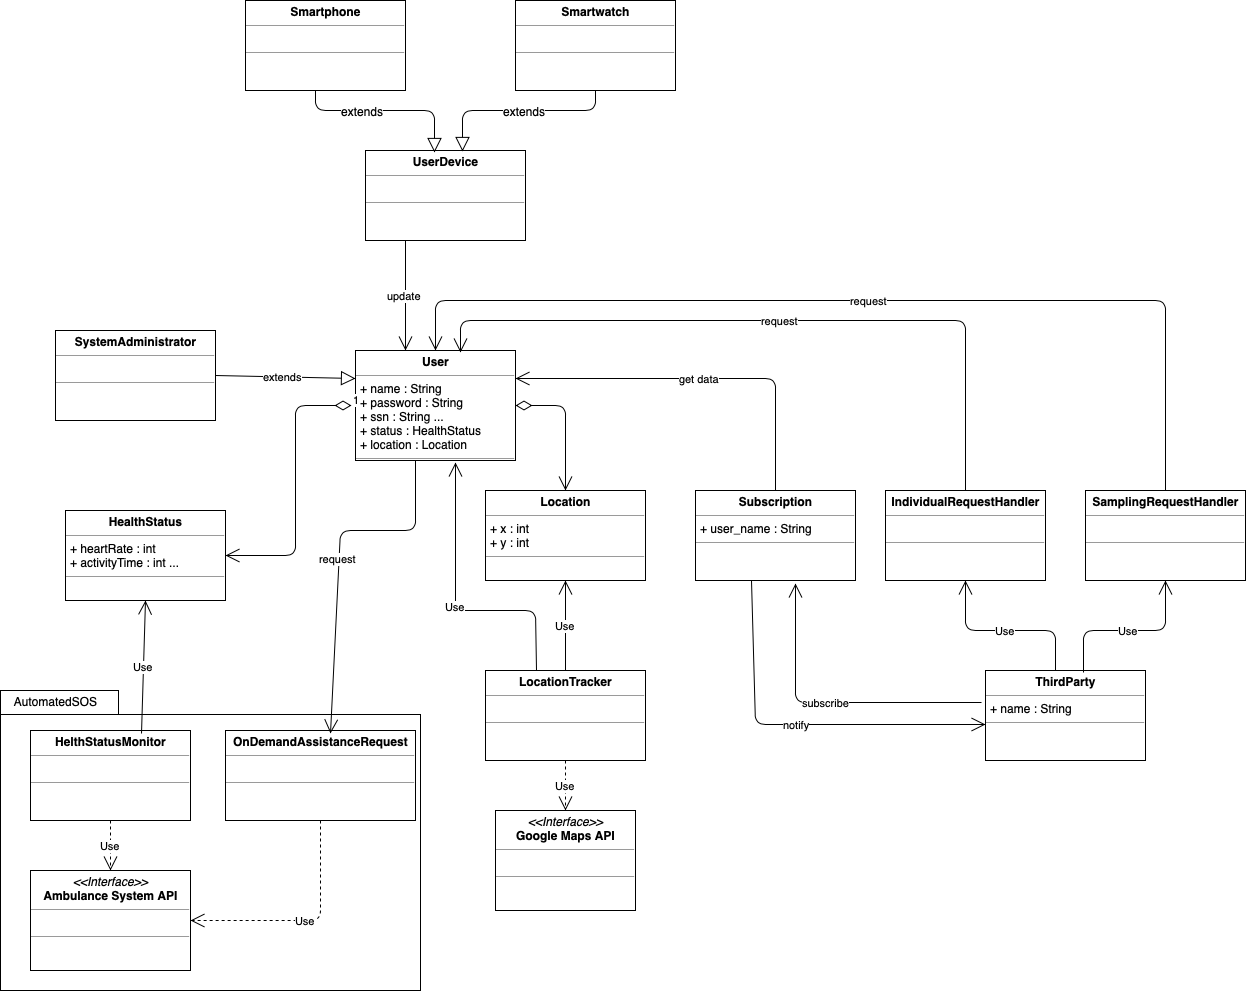
\includegraphics[width=1.25\linewidth]{Images/uml}
				\caption{UML Class Diagram}
				\label{fig:uml}
			\end{figure}
			\newpage
			Here below two UML Statechart Diagrams, one for the User and one for the Third Party, are provided to describe the state transition of the two actors according to external events: 
			\begin{figure}[H]
				\centering
				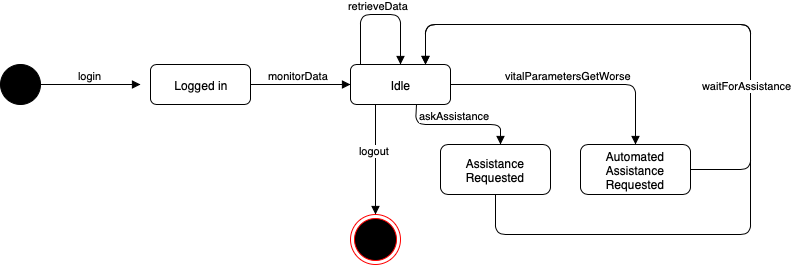
\includegraphics[width=1.0\linewidth]{Images/statechart_user}
				\caption{User Statechart Diagram}
				\label{fig:statechart_user}
			\end{figure}
			\begin{figure}[H]
				\centering
				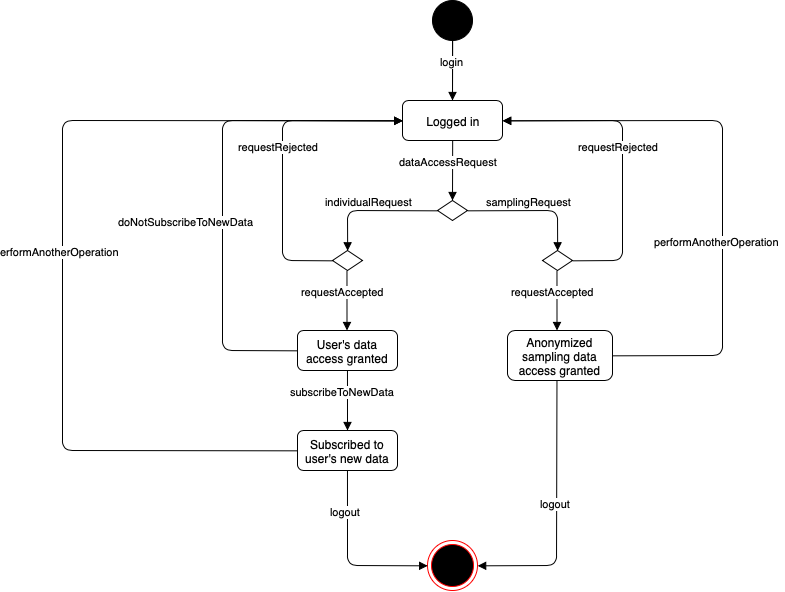
\includegraphics[width=1.0\linewidth]{Images/statechart_third_party}
				\caption{Third Party Statechart Diagram}
				\label{fig:statechart_third_party}
			\end{figure}

		\newpage
		\subsection{Product Functions}
			According to the goals defined for the current system, we can highlight briefly the main functions of the Application, that can be divided in 4 groups which are the following:
			\begin{itemize}
				\item \texttt{Registration and Login}: This functionality lets a Visitor (either a Visitor or a Third Party) to register to TrackMe and therefore be able to Login.
				\item \texttt{Data Monitoring}: Data4Help periodically monitors Users' parameters, such as physical activity, distance and recurred path, sleep, heartbeat and so on.
				\item \texttt{Data Access and Update}: Users registered to TrackMe can either visualize their data or update it. Users will also be able to update the list of third parties that can access to their data.
				Moreover, Third Parties can have access to some Users' data after their approval and can request samplings that return anonymized data of a group of people satisfying some filters.
				\item \texttt{Automated Assistance}: This functionality is very crucial for the system. It allows registered Users to receive an assistance when it's necessary. Elderly people will be automatically subscribed to this service, but all the other users will be able to choose during the registration process. In addition TrackMe will also be able to provide a form of on-demand assistance request that each user can ask for when he feels necessary.
			\end{itemize}
	
		\newpage
		\subsection{User Characteristics}
		\begin{itemize}
			\item \texttt{Visitor}: a person/third party visiting TrackMe without being registered. He can only proceed to registration in oder to actually use system services, otherwise he can't have access to any service or data.
			\item \texttt{Registered User}: called simply \texttt{user} in this document. A person who registered himself to TrackMe, sharing his personal data. He can login to the system through provided credentials to exploit full services.
			\item \texttt{Third Party User}: called simply \texttt{third party} in this document. A company or invidual using the platform for some statistical goal or to offer assistance to registered users.
			\item \texttt{System Administrator}: doesn't require to register himself. Makes sure there are no issues in the interaction between users and third parties, guaranteeing a certain level of security. He can report a misuse of the system functionalities.
			\item \texttt{Ambulance Dispatcher}: called simply \texttt{dispatcher} in this document. An external individual to the system, whose role is to dispatch an ambulance to assist specific users.
		\end{itemize}

		%\subsection{Assumptions, Dependencies and Constraints}
		\subsection{Domain Assumptions}
			\begin{itemize}
				\item {\textbf[}\textbf{D1}{\textbf]}: The Social Security Number is unique.
				\item {\textbf[}\textbf{D2}{\textbf]}: Users are assumed to provide a valid Mobile Number and e-mail.
				\item {\textbf[}\textbf{D3}{\textbf]}: The verification message sent by SMS/e-mail will be certainly received by the User/Third Party.
				\item {\textbf[}\textbf{D4}{\textbf]}: Users' devices are up and running in order to retrieve and process vital parameters.
				\item {\textbf[}\textbf{D5}{\textbf]}: Parameters periodically received by Users' devices are assumed to have a good accuracy.
				\item {\textbf[}\textbf{D6}{\textbf]}: Personal information provided by Users' are assumed to be correct.
				\item {\textbf[}\textbf{D7}{\textbf]}: Users provide correct clinical data (such as blood group, allergies, etc.).
				\item {\textbf[}\textbf{D8}{\textbf]}: Users' devices support the GPS technology.
				\item {\textbf[}\textbf{D9}{\textbf]}: Users' devices support the Mobile Application.
				\item {\textbf[}\textbf{D10}{\textbf]}: Users' devices support sensors for retrieving health parameters.
				\item {\textbf[}\textbf{D11}{\textbf]}: Users' devices communicate through the Internet.
				\item {\textbf[}\textbf{D12}{\textbf]}: In case of emergency, all relevant data relative to a specific individual are correctly reported to the Ambulance Dispatching System.
				\item {\textbf[}\textbf{D13}{\textbf]}: The Ambulance Dispatching System is always running and available.
				\item {\textbf[}\textbf{D14}{\textbf]}: The time spent by an ambulance to reach a defined location is as low as possible.
			\end{itemize}

	\newpage
	\section{Specific Requirements}
		\subsection{External Interface Requirements}
				\subsubsection{User Interfaces (UI)}
					The following mockups represent a basic idea of how the Mobile Application and the Web Interface are supposed to look like.
					\\ \\
					Users can access to complete TrackMe functionalities through the smartphone application, while the smartwatch one will only support a subset of the system's services.
					\\ \\
					On the other side, TrackMe provides a Web Interface for Third Parties. Here they can exploit all the functionalities at their disposal, such as the request of a sampling according to some parameters.
					\begin{figure}[h]
						\centering
						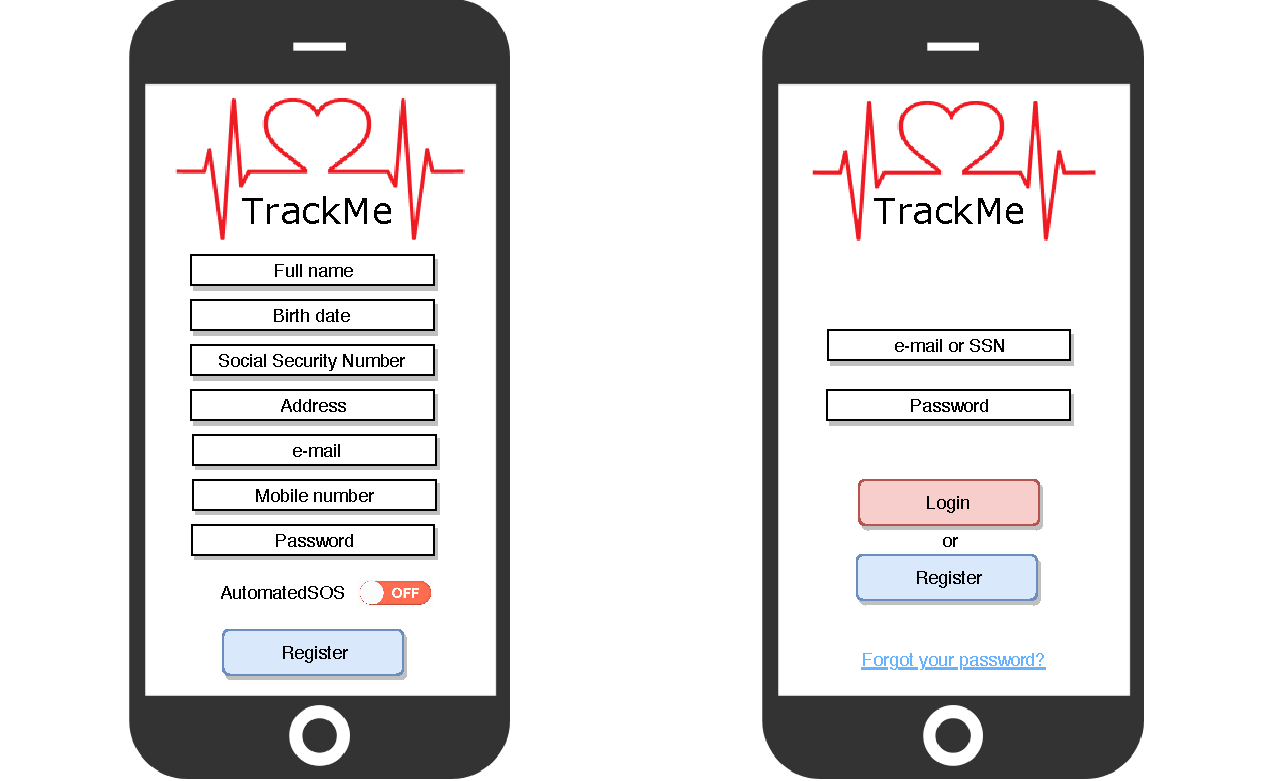
\includegraphics[width=1.0\linewidth]{Images/login-registration.pdf}
						\caption{Mobile App registration form and login page.}
						\label{fig:login-registration}
					\end{figure}
					\begin{figure}[H]
						\centering
						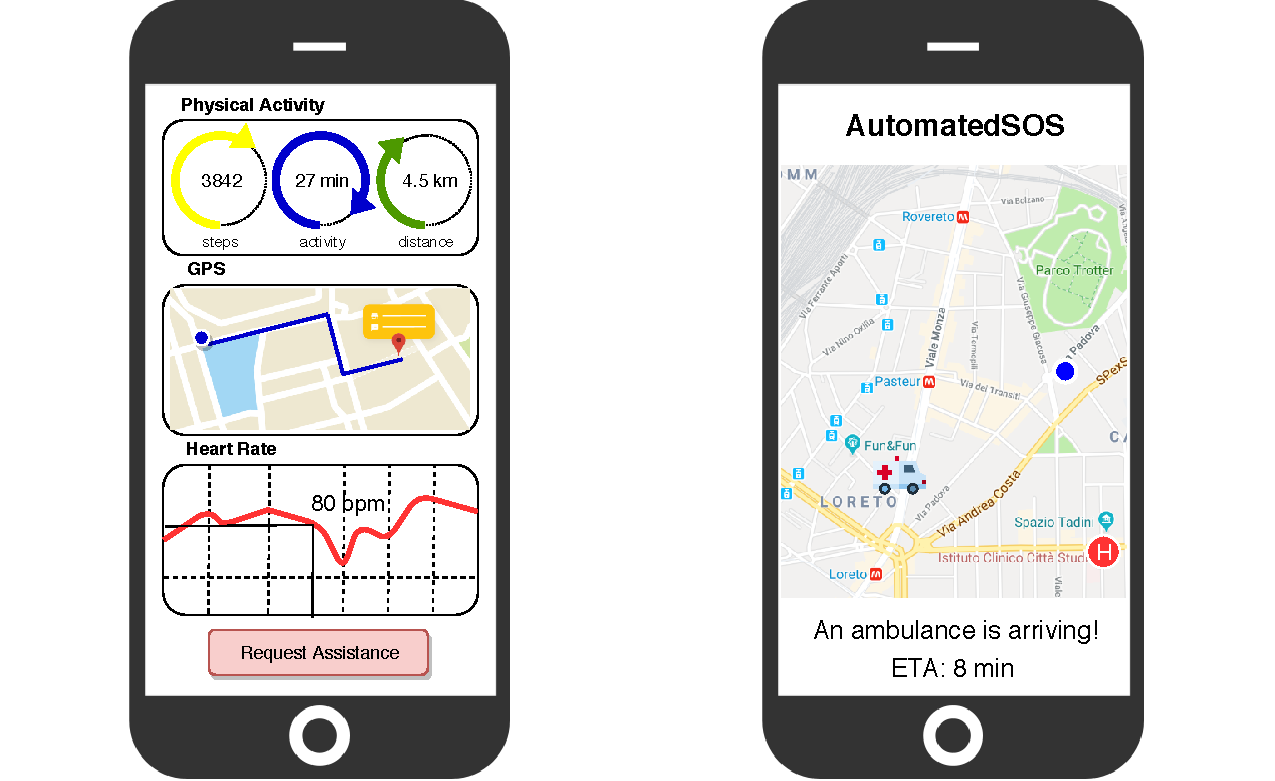
\includegraphics[width=1.0\linewidth]{Images/pages}
						\caption{Mobile App homepage with activity data and AutomatedSOS interface during an ambulance request.}
					\end{figure}
					\begin{figure}[H]
						\centering
						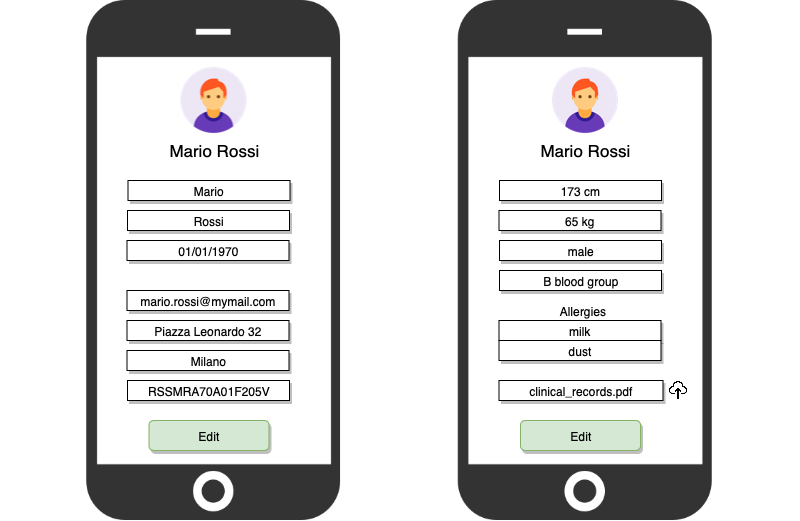
\includegraphics[width=1.0\linewidth]{Images/data-pages}
						\caption{Personal information and clinical data pages.}
						\label{fig:data-pages}
					\end{figure}
					\begin{figure}[H]
						\centering
						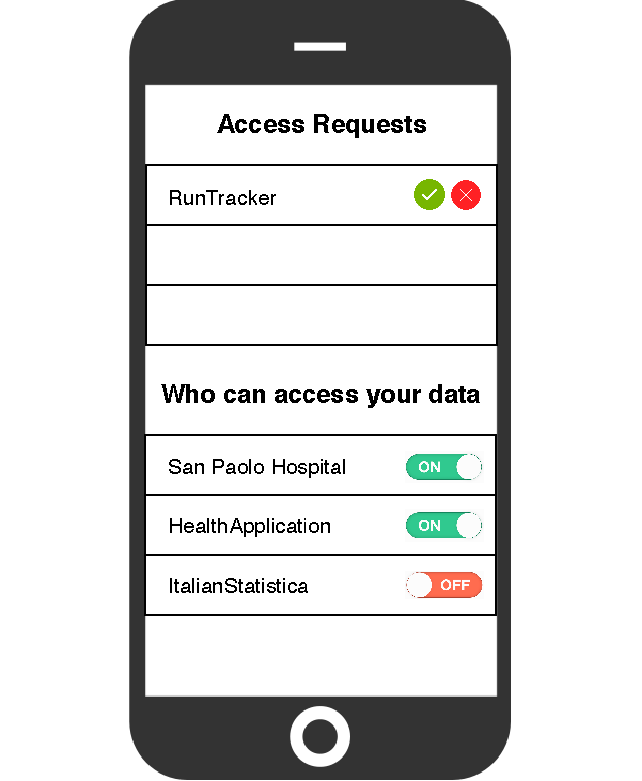
\includegraphics[width=0.6\linewidth]{Images/access_management}
						\caption{Data access management page.}
						\label{fig:access_management}
					\end{figure}
					\begin{figure}[H]
						\centering
						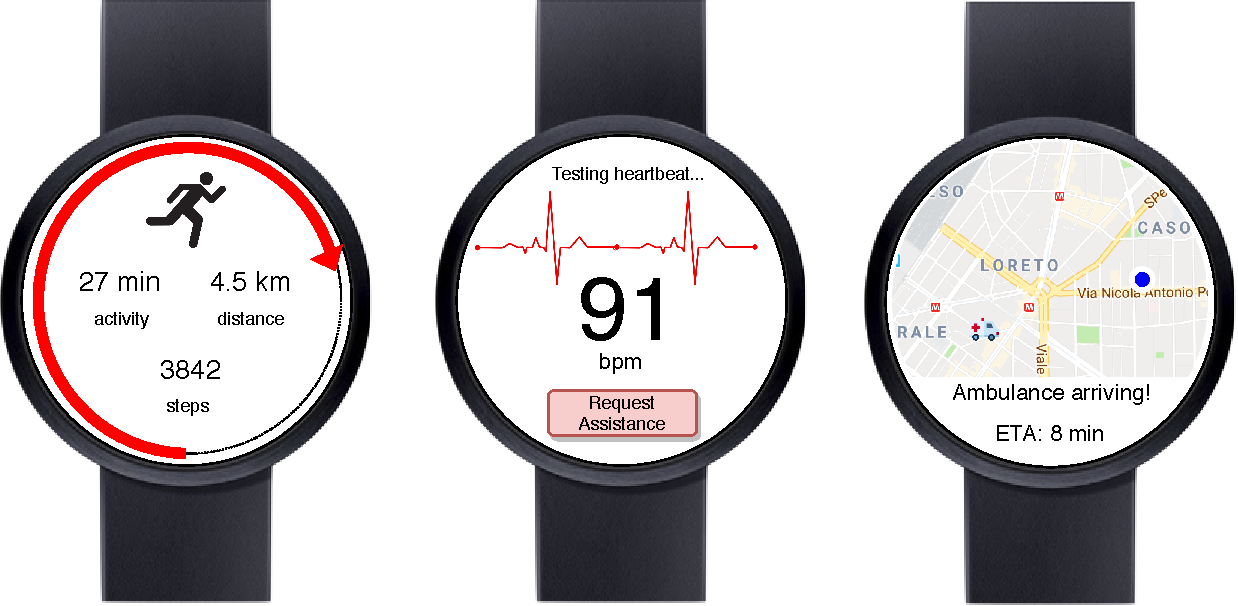
\includegraphics[width=1.0\linewidth]{Images/smartwatch}
						\caption{Smartwatch UI homepage with activity data, heartbeat testing page and AutomatedSOS interface during an ambulance request.}
						\label{fig:smartwatch}
					\end{figure}
					\begin{figure}[H]
						\centering
						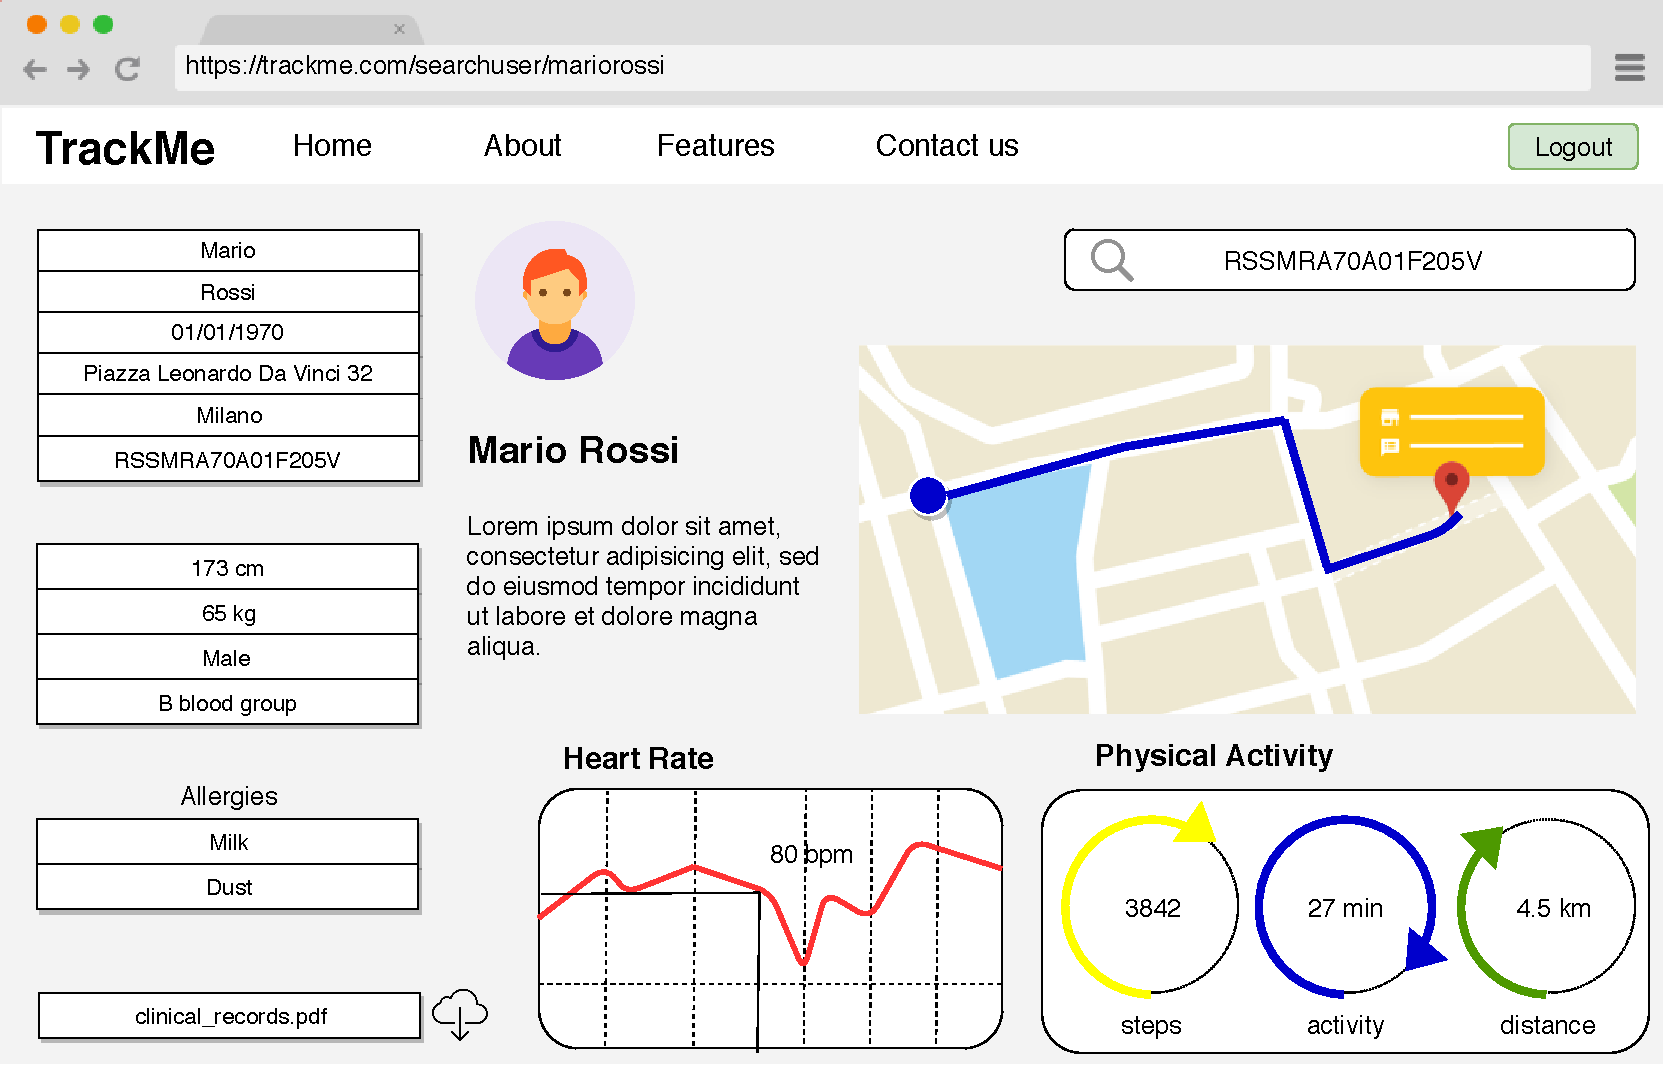
\includegraphics[height=0.6\linewidth]{Images/webapp_search_user}
						\caption{Web App UI when a Third Party searches a User that has already accepted its request (data access).}
						\label{fig:webapp_search_user}
					\end{figure}
					\begin{figure}[H]
						\centering
						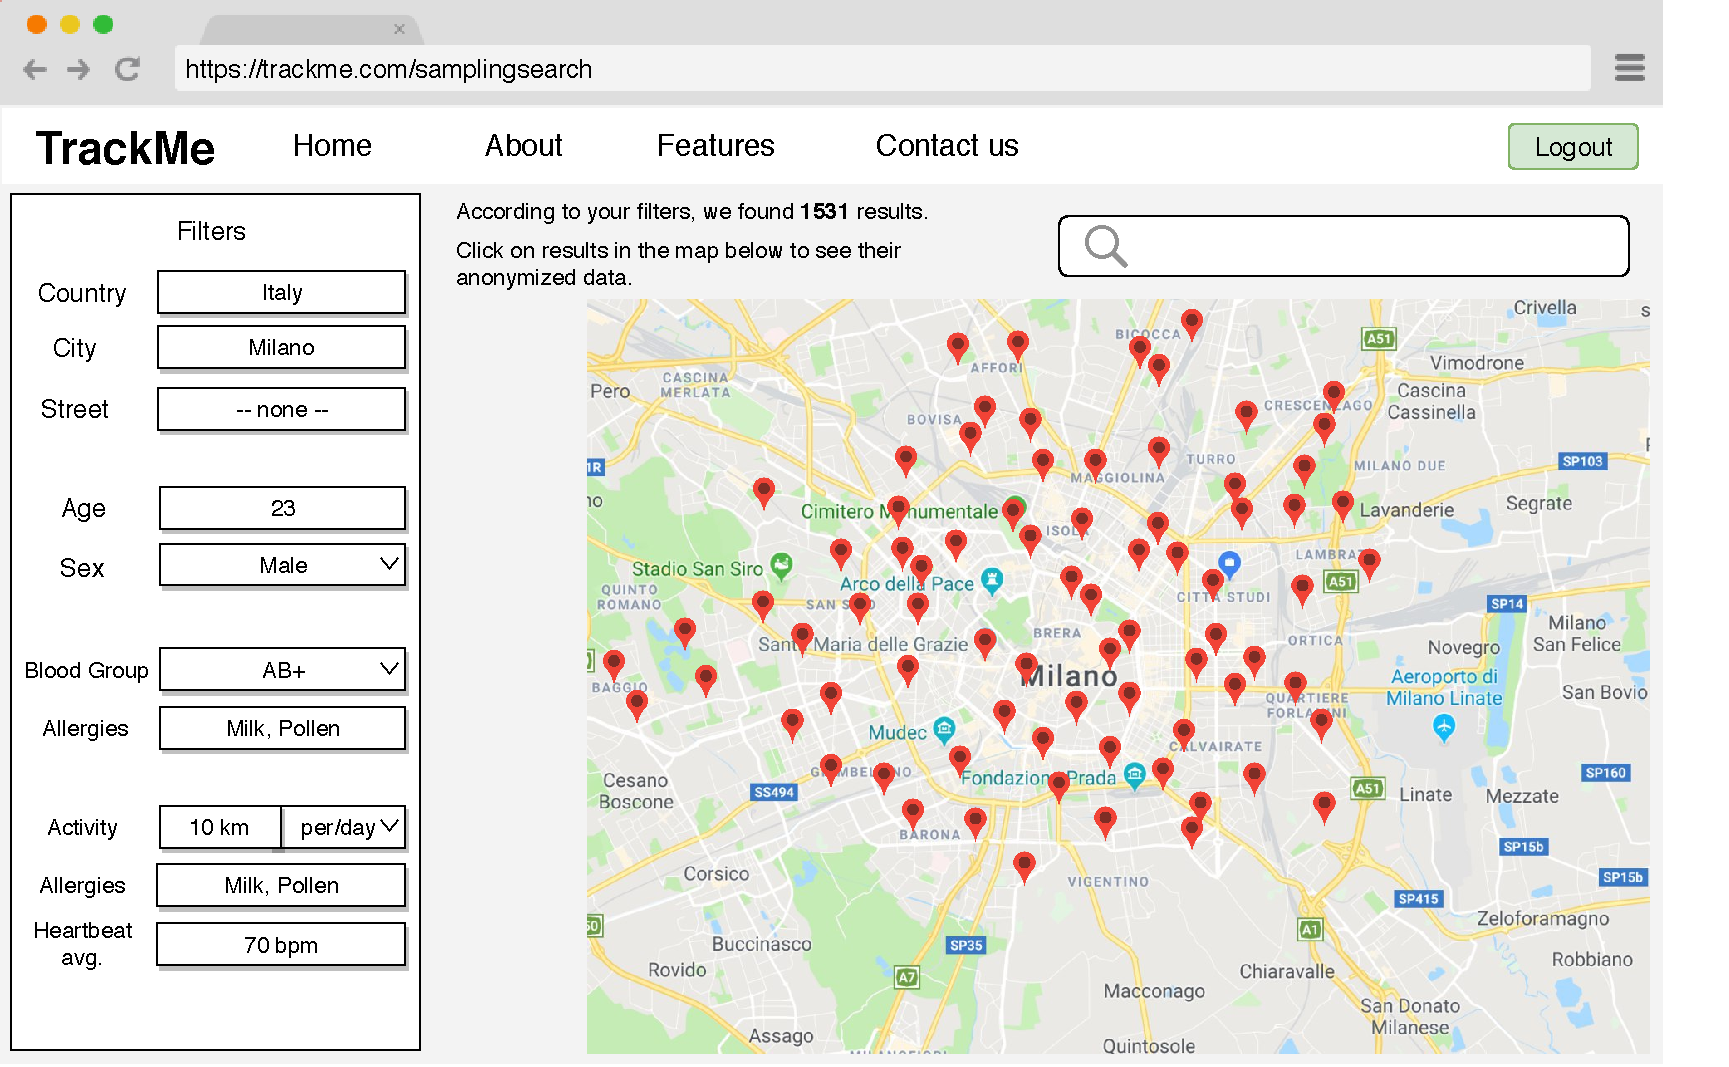
\includegraphics[height=0.6\linewidth]{Images/webapp_sampling}
						\caption{Web App sampling search results.}
						\label{fig:webapp_sampling}
					\end{figure}

	\newpage
	\subsubsection{Hardware Interfaces}
		Since the application must run over the Internet, all the hardware shall require to connect network will be an hardware interface for the system, both server and client side.
		\begin{itemize}
			\item Server-side: e.g. Modem, WAN - LAN, Ethernet Cross-Cable.
			\item Client-side: e.g. Wi-Fi 802.11ac+ antenna, 3G/4G antenna. Moreover, bluetooth antenna and body sensors will be needed to use all services provided by Data4Help and AutomatedSOS. 
		\end{itemize}
	\subsubsection{Software Interfaces}
		TrackMe will provide an API for third parties, besides the already mentioned Web Application Interface.\\
		More specifically, it will provide an API that allows third parties to access the entire set of functionalities provided by the Data4Help system. In such a way third party companies and applications can embed in their system the functionalities concerning with the individual access requests and sampling requests. 
		
	\subsubsection{Communication Interfaces}
			Since the TLS versions 1.0 and 1.1 will not be more supported, TrackMe must rely on the newer TLS version 1.3, released in 2018, to guarantee the best security possible, at least during the HTTPS connections involving messages carrying credentials or other sensible data.
			\\ \\
			Furthermore, Bluetooth connectivity is required in order to interface between themselves Users' devices. Indeed, the Mobile Application running on a smartphone needs to communicate with a smartwatch (if this last device doesn't have a GPS module and internet connectivity) in order to fully exploit TrackMe's functionalities. The newest Bluetooth 5.0 will be preferred, even though older versions of the standard have to be supported, since the majority of devices don't support the latest one yet.

	\newpage
	\subsection{Scenarios}
	\subsubsection*{Scenario 1 - Registration}
		Marco saw the advertisement of TrackMe and decided to download the mobile application in order to exploit in a useful way his new smartwatch. After opening the new app, he is asked to fill a form with all his personal information, full name, date of birth, mobile number, SSN, etc. To proceed with his registration, after all fields have been filled, Marco clicks on the "Register" button and, as soon as he does, he receives an SMS on his mobile phone confirming the positive outcome of his operation. Marco is now a Registered User of TrackMe: he can login to update his clinical information and benefit of all functionalities of the application.

	\subsubsection*{Scenario 2 - Automatic Ambulance Request}
		Maria is a 76 years old User of TrackMe, so she can benefit of the AutomatedSOS service. Thanks to this functionality, the system checks periodically her heart rate. During a relax time, Maria's heart rate get so low that her heart risks to stop. Luckily she always wears a smartwatch on her wrist, because she's aware of the utility and importance of TrackMe's monitoring. In fact, as soon as her heart rate gets lower than 30 bpm, AutomatedSOS sends an assistance request to the Ambulance Dispatching System, notifying Maria about the estimated time of arrival of the aid team.

	\subsubsection*{Scenario 3 - On-Demand Ambulance Request}
		A sport addict user such as John always goes out during the morning to have a run in the park.
		In the last period he didn't have time to train himself so much as before and now he has more difficulties. Coming back to home, he starts feeling weak. He measure his pressure values and notices that they are lower than their normal level. To speed up the operation and to avoid calling the ambulance service, he logs in his TrackMe account and in the homepage he clicks on "Request assistance". The application confirms that the request has been successfully sent and notifies Jhon about the Estimated Time of Arrival of the ambulance.

	\subsubsection*{Scenario 4 - Search for a User}
		San Paolo, a hospital located in Milan is looking for a blood donor, whose  group is O- in order to help out a patient with a blood transufion. According to medicine, a recipient with blood type O- can only receive blood from blood group O- only. Therefore, San Paolo, which is registered to TrackMe as a Third Party, is searching for Users whose blood group matches with the patient one.
		Franco, a registered User to TrackMe and a patient of San Paolo, receives a request in which there is a brief description about the research of a blood donor. Knowing about the importance of such fact and that he has blood group O- (which is the one requested for the blood transfusion), Franco accepts the request.

	\subsubsection*{Scenario 5 - Anonymous Sampling}
		ItalianStatistica is a big company that performs statistical analysis on the italian territory studying the differences between some geographical areas. For a new analysis on Milan's population, ItalianStatistica decides to retrieve samples from the Data4Help database. After the registration the company can perform anonymous samplings on the people living in Milan. Since asking for how many people with blue eyes and younger than 15 live in the city center results in sampling than 1000 individuals, Data4Help refuses such a request. In order to produce a sampling, ItalianStatistica extends the search to the entire municipality. In this way, a group of more than 1000 individuals is found and the sample with all relevant data is made accessible to the company.

	\newpage

	\subsection{Functional Requirements}

	\subsubsection*{{[}{G1}{]}: Allow visitors to easily register in the system and later to login}
	\begin{itemize}
		\begin{itemize}
			\item {[D1]}: The Social Security Number is unique.
			\item {[D2]} Users are assumed to provide a valid Mobile Number and e-mail.
			\item {[D3]}: The verification message sent by SMS/e-mail will be certainly received by the User/Third Party.
			\\\\
			\item {[R1]}: The system must allow the Visitor to provide credentials and personal data.
			\item {[R2]}: The system must verify the correspondance between the SSN provided by the Visitor and their personal information.
			\item {[R3]}: The system must let the Visitor to verify the account with an e-mail/SMS verification.
			\item {[R4]}: The system must verify that there are no other registered Users/Third Parties with the same e-mail/SSN.
			\item {[R5]}: In order to register successfully a Third Party, the system must oblige it to accept users data privacy conditions.
		\end{itemize}
	\end{itemize}
	\subsubsection*{{[}{G2}{]}: Allow Users to share personal information/health parameters}
	\begin{itemize}
		\begin{itemize}
			\item {[D4]}: Users' devices are up and running in order to retrieve and process vital parameters.
			\item {[D5]}: Parameters periodically received by Users' devices are assumed to have a good accuracy.
			\item {[D6]}: Personal information provided by Users' are assumed to be correct.
			\item {[D7]}: Users provide correct clinical data (such as blood group, allergies, etc.).
			\item {[D8]}: Users' devices support the GPS technology.
			\item {[D9]}: Users' devices support the Mobile Application.
			\item {[D10]}: Users' devices support sensors for retrieving health parameters.
			\item {[D11]}: Users' devices communicate through the Internet.
			\\ \\
			\item {[R6]}: Users locations must be retrieved by GPS.
			\item {[R7]}: The system must allow the Users to update their personal data.
			\item {[R8]}: The system must allow the Users to upload their medical records (such as blood group).
		\end{itemize}
	\end{itemize}
	\subsubsection*{{[}{G3}{]}: Allow Third Parties to access information shared by the Users}
	\begin{itemize}
		\item {[G3.1]}: Allow Third Parties to access information of specific individuals.
		\begin{itemize}
			\item {[R9]}: The system must allow Third Parties to search Users through their SSN's.
			\item {[R10]}: The system must allow Third Parties to send requests in order to access specific data.
			\item {[R11]}: The system must allow Users either to accept or refuse Third Parties' requests.
		\end{itemize}

		\item {[G3.2]}: Allow Third Parties to access anonymized information and parameters of groups of individuals.
		\begin{itemize}
			\item {[R12]}:The system must allow Third Parties to perform samplings according to some parameters (such as Geographical ones).
			\item {[R13]}: The system must anonymize sampling result data.
			\item {[R14]}: The system must accept sampling if and only if results are related to more than 1000 Users.
		\end{itemize}

		\item {[G3.3]}: Allow Third Parties to subscribe to new information of a specific individual and to receive it.
		\begin{itemize}
			\item {[R15]}: If a User accepts a requests, the system must allow Third Parties to store and access the previously saved data.
			\item {[R16]}: The system must show Third Parties new data whenever they are available.
		\end{itemize}
	\end{itemize}
	\subsubsection*{{[}{G4}{]}: Guarantee users an assistance service when necessary}
		\begin{itemize}
			\item {[G4.1]}: Guarantee the elderly users to receive an immediate assistance by an ambulance in case of high risk disease.
			\begin{itemize}
				\item {[D5]}: Data periodically received by Users' devices are assumed to have a good accuracy.
				\item {D8}: Users' devices support the GPS technology.
				\item {[D10]}: Users' devices must support sensors for retrieving health parameters.
				\item {[D12]}: In case of emergency, all relevant data relative to a specific individual are correctly reported to the Ambulance Dispatching System.
				\item {[D13]}: The Ambulance Dispatching System is always running and reliable.
				\item {[D14]}: The time spent by an ambulance to reach a defined location is as low as possible.
				\\ \\
				\item {[R17]}: The AutomatedSOS service is automatically activated during the registration process if the User is over 60.
				\item {[R18]}: The system must notify the Ambulance Dispatching System as soon as possible (within 5 seconds), when it is needed.
				\item {[R19]}: When the Ambulance Dispatching System is notified, the system sends all the User's clinical parameters.
			\end{itemize}
			\item {[G4.2]}: Allow users to request on-demand ambulance assistance.
			\begin{itemize}
				\item {[D5]}: Parameters periodically received by Users' devices are assumed to have a good accuracy.
				\item {D8}: Users' devices support the GPS technology.
				\item {[D12]}: In case of emergency, all relevant data relative to a specific individual are correctly reported to the Ambulance Dispatching System.
				\item {[D13]}: The Ambulance Dispatching System is always running and reliable.
				\item {[D14]}: The time spent by an ambulance to reach a defined location is as low as possible.
				\\ \\
				\item {[R18]}: The system must notify the Ambulance Dispatching System as soon as possible (within 5 seconds), when it is needed.
				\item {[R19]}: When the Ambulance Dispatching System is notified, the system sends all the User's clinical parameters.
				\item {[R20]}: The system must avoid abuses of on-demand assistance requests functionality.
			\end{itemize}
		\end{itemize}
	
	\subsubsection*{{[}{G5}{]}: Guarantee the preservation of the privacy of the Users}
	\begin{itemize}
		\begin{itemize}
			\item {[R5]}: In order to register successfully a Third Party, the system must oblige it to accept data privacy conditions.
			\item {[R14]}: The system must accept sampling if and only if results are related to more than 1000 Users.
			\item {[R21]}: A Third Party can access data and parameters of a specific User if and only if he/she accepts the request.
			\item {[R22]}: The system must allow Users to check the list of third parties accessing their data.
			\item {[R23]}: The system must allow the User to enable/disable data access by third parties.
			\item {[R24]}: The system must implement some form of accurate access control on databases.
		\end{itemize}
	\end{itemize}

	\newpage
	\subsection{Use Case Diagram}
	Here is represented a Use Case diagram representing all functionalities accessible by each actor:
	\begin{figure}[h]
		\centering
		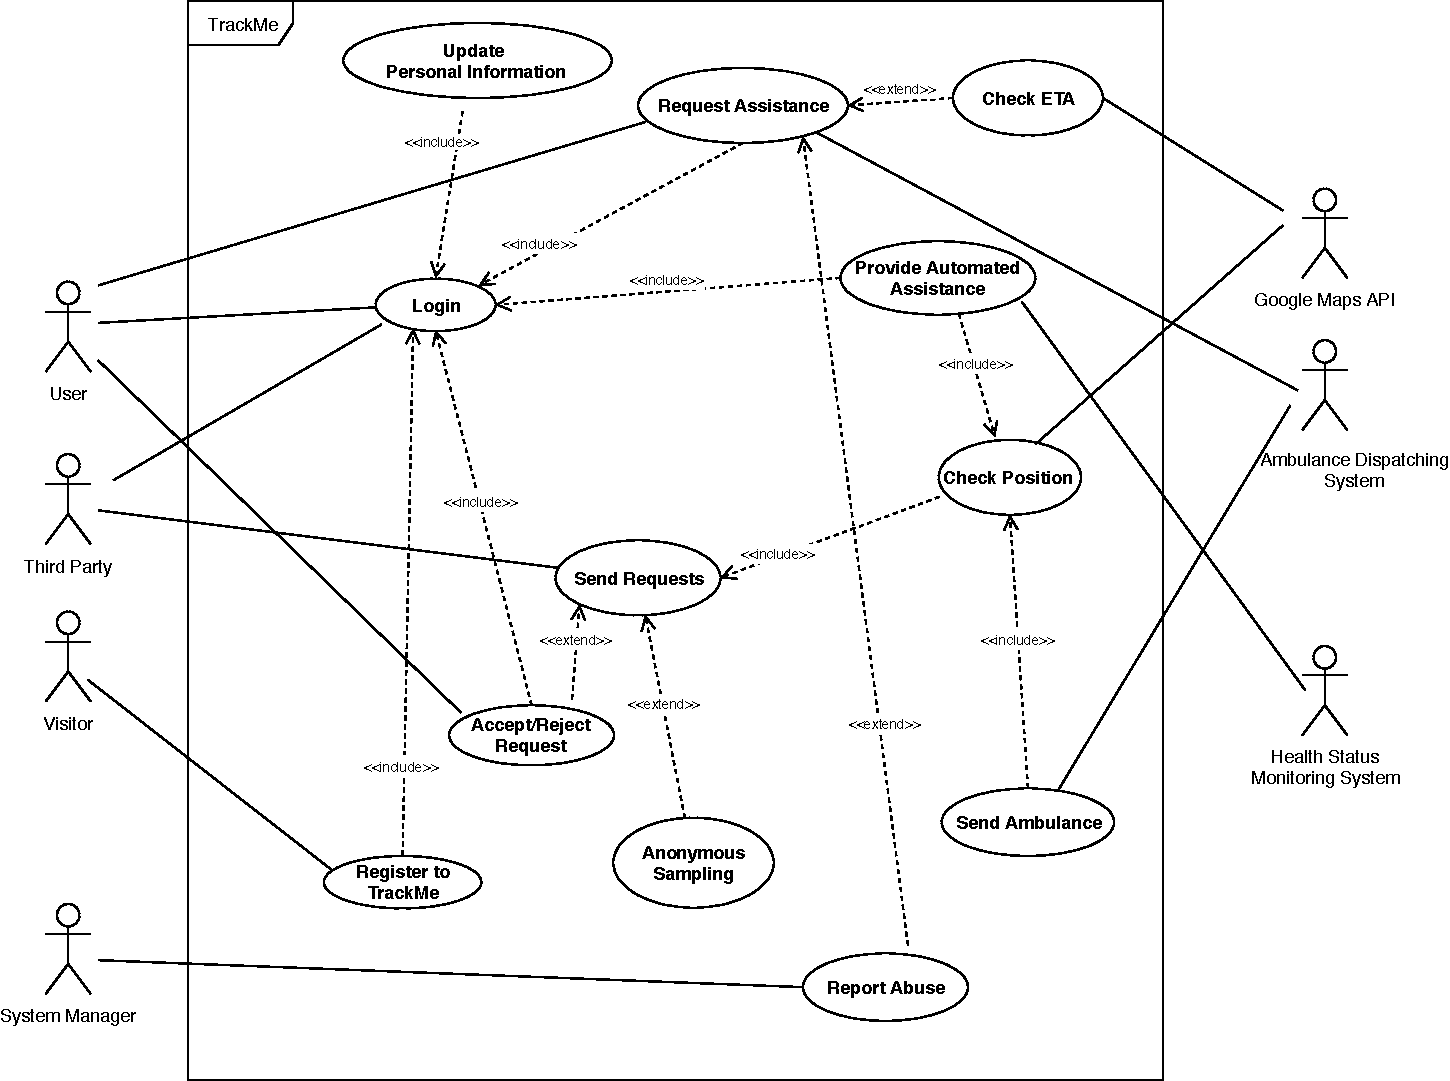
\includegraphics[width=1.25\linewidth]{Images/use_case_diagram}
		\label{fig:use_case_diagram}
	\end{figure}

	\newpage
	\subsection{Use cases}
		\subsubsection{Visitor Registration}
		\begin{center}
			\begin{tabular}{| c | l |}
				\hline
				\textbf{NAME} & Register to TrackMe \\
				\hline
				\textbf{ACTOR} & Visitor \\
				\hline
				\textbf{GOALS} & [G1] \\
				\hline
				\textbf{ENTRY CONDITIONS} & The Visitor has installed \\
				&	the Application on his/her Mobile device \\ \hline
				\textbf{EVENTS FLOW}  &
				1. Fill all mandatory fields in the Registration Form\\
				&2. The visitor clicks on "Register" button\\
				&3. The system checks data validity\\
				&4. The system sends an SMS as confirmation\\
				&5. The system saves Users' data\\
				\hline
				\textbf{EXIT CONDITIONS}  & The Vistor has successfully registered to TrackMe\\ \hline
				\textbf{EXCEPTIONS} &
				1. The User is already registered\\
				&2. The e-mail is already registered\\
				&3. The Mobile Number is already registered\\
				&4. The SSN provided is invalid\\
				&5. Some mandatory fields are not filled\\
				\hline
			\end{tabular}
		\end{center}

		\subsubsection{User Login}
		\begin{center}
			\begin{tabular}{| c | l |}
				\hline
				\textbf{NAME} & User Login \\
				\hline
				\textbf{ACTOR} & User \\
				\hline
				\textbf{GOALS} & [G1] \\
				\hline
				\textbf{ENTRY CONDITIONS} & The User is in the Login page \\ \hline
				\textbf{EVENTS FLOW}  &
				1. The User enters e-mail or SSN\\
				&2. The User enters the password\\
				&3. The User clicks on "Login" button\\
				&4. The system checks the correctness of the credentials\\
				\hline
				\textbf{EXIT CONDITIONS}  & The User has successfully logged in \\ \hline
				\textbf{EXCEPTIONS} &
				1. The User is not registered\\
				&2. The e-mail is wrong\\
				&3. The SSN is wrong\\
				&4. The password is wrong\\
				&5. Some mandatory fields are not filled\\
				\hline
			\end{tabular}
		\end{center}

		\subsubsection{Third Party Login}
		\begin{center}
			\begin{tabular}{| c | l |}
				\hline
				\textbf{NAME} & Third Party Login \\
				\hline
				\textbf{ACTOR} & Third Party \\
				\hline
				\textbf{GOALS} & [G1] \\
				\hline
				\textbf{ENTRY CONDITION} & The Third Party is in the Login page \\ \hline
				\textbf{EVENTS FLOW}  &
				1. The Third Party enters e-mail or SSN\\
				&2. The Third Party enters the password\\
				&3. The Third Party clicks on "Login" button\\
				&4. The Third Party systems checks the correctness\\
				& of the credentials\\
				\hline
				\textbf{EXIT CONDITIONS}  & The Third Party has successfully logged in \\ \hline
				\textbf{EXCEPTIONS} &
				1. The Third Party is not registered\\
				&2. The e-mail is wrong\\
				&3. The SSN is wrong\\
				&4. The password is wrong\\
				&5. Some mandatory fields are not filled\\
				\hline
			\end{tabular}
		\end{center}

		\subsubsection{Update Personal Information}
		\begin{center}
			\begin{tabular}{| c | l |}
				\hline
				\textbf{NAME} & Update Personal Information \\
				\hline
				\textbf{ACTOR} & User \\
				\hline
				\textbf{GOALS} & [G2] \\
				\hline
				\textbf{ENTRY CONDITION} & The User is in the personal data page after Login\\ \hline
				\textbf{EVENTS FLOW}  &
				1. The User clicks on "Edit" button\\
				&2. The User changes his/her personal information \\
				&3. The User confirms the changes\\
				&4. The system checks that the inserted values are\\
				& appropriate\\
				\hline
				\textbf{EXIT CONDITIONS}
				& The User has successfully edited his/her \\
				& personal information \\ \hline
				\textbf{EXCEPTIONS} &
				 The User edited one or more fields in an \\
				& inappropriate way (e.g. added a non-existing address)\\
				\hline
			\end{tabular}
		\end{center}
	
		\newpage
		\subsubsection{Manage Third Party Accesses}
		\begin{center}
			\begin{tabular}{| c | l |}
				\hline
				\textbf{NAME} & Manage Third Party Accesses \\
				\hline
				\textbf{ACTOR} & User \\
				\hline
				\textbf{GOALS} & [G5] \\
				\hline
				\textbf{ENTRY CONDITION} & The User is in the data access management page after \\
				& Login\\ 
				\hline
				\textbf{EVENTS FLOW}  &
				1. The User clicks on "Edit" button\\
				&2. The User changes a third party's access privilege from \\
				&"On" to "Off" \\
				&3. The User confirms the changes\\
				&4. The system updates the third party's privileges \\ 
				\hline
				\textbf{EXIT CONDITIONS}
				& The User has successfully updated the list of third parties \\
				& that can access to his/her data\\ \hline
				\textbf{EXCEPTIONS} &
				None \\
				\hline
			\end{tabular}
		\end{center}
	
		\subsubsection{Provide Automated Assistance}
		\begin{center}
			\begin{tabular}{| c | l |}
				\hline
				\textbf{NAME} & Provide Automated Assistance \\
				\hline
				\textbf{ACTOR} & Health Status Monitor \\
				\hline
				\textbf{GOALS} & [G4.1] \\
				\hline
				\textbf{ENTRY CONDITION} & Some User's parameters are below a certain threshold \\ \hline
				\textbf{EVENTS FLOW}  &
				1. The system detects that some parameters are below a \\
				& threshold\\
				&2. The system requests an ambulance to assist the user\\
				&3. The system retrieves user's location and data and\\
				&forwards them to the Ambulance Dispatching System,\\
				& requesting an ambulance \\
				&4. The Ambulance System confirms the availability\\
				&5. The Ambulance System communicates the ETA\\
				\hline
				\textbf{EXIT CONDITIONS}  & An ambulance has been sent to the user's location \\ \hline
				\textbf{EXCEPTIONS} &
				GPS is not active on User's device\\
				\hline
			\end{tabular}
		\end{center}
		\textbf{Note}: with the expression "Health Status Monitor" we mean the set of TrackMe components that will handle the functionalities of monitoring users' vital parameters. So, indirectly, it can be considered as the actor itself of this use case, since it will interact with the Ambulance Dispatching System.
	
		\newpage
		\subsubsection{On-Demand Assistance Request}
		\begin{center}
			\begin{tabular}{| c | l |}
				\hline
				\textbf{NAME} & Request Assistance \\
				\hline
				\textbf{ACTOR} & User \\
				\hline
				\textbf{GOALS} & [G4.2] \\
				\hline
				\textbf{ENTRY CONDITION} & The User is in the HomePage after Login\\ \hline
				\textbf{EVENTS FLOW}  &
				1. The User clicks on "Request Assistance" button\\
				&2. The User confirms the operation when it is asked\\
				&3. The system requests an ambulance to assist the user\\
				&4. The system retrieves user's location and data and\\
				&forwards them to the Ambulance Dispatching System,\\
				& requesting an ambulance \\
				&5. The Ambulance System confirms the availability\\
				&6. The Ambulance System communicates the ETA\\
				\hline
				\textbf{EXIT CONDITIONS}  & The User has successfully requested Assistance\\
				& and an ambulance has been sent to the user's location\\ \hline
				\textbf{EXCEPTIONS} &
				GPS is not active on User's device\\ \hline
				\textbf{SPECIAL REQ.} &
				The request must be processed in less than 5 seconds.\\
				\hline
			\end{tabular}
		\end{center}
	
		\subsubsection{Report Abuse}
		\begin{center}
			\begin{tabular}{| c | l |}
				\hline
				\textbf{NAME} & Report Abuse \\
				\hline
				\textbf{ACTOR} & System Manager \\
				\hline
				\textbf{GOALS} & [G4.2] \\
				\hline
				\textbf{ENTRY CONDITION} & The System Manager notices an abuse\\ 
				& of the assistance request system\\
				\hline
				\textbf{EVENTS FLOW}  &
				1. The System Manager signals the User that is \\
				& misusing the service\\
				&2. The system notifies the User that he/she will no more\\
				& be able to exploit the on-demand assistance request\\
				& service\\
				&3. The system inserts the User in the list of the users\\
				& that don't have access to such a service\\
				\hline
				\textbf{EXIT CONDITIONS}  & The User is no more able to use the on-demand\\
				& assistance request service\\ 
				\hline
				\textbf{EXCEPTIONS} & None \\
				\hline
			\end{tabular}
		\end{center}

		\newpage
		\subsubsection{Accept Access Request}
		\begin{center}
			\begin{tabular}{| c | l |}
				\hline
				\textbf{NAME} & Accept Request \\
				\hline
				\textbf{ACTOR} & User \\
				\hline
				\textbf{GOALS} & [G3.1] \\
				\hline
				\textbf{ENTRY CONDITION} & The User has received an access request\\
				& from a Third Party\\  \hline
				\textbf{EVENTS FLOW}  &
				1. The User receives a request from a Third Party\\
				&2. The User clicks on "Accept" button\\
				\hline
				\textbf{EXIT CONDITIONS}  & The User has successfully accepted the request\\ 
				& and the Third Party can access to his/her data\\
				\hline
				\textbf{EXCEPTIONS} &
				None\\
				\hline
			\end{tabular}
		\end{center}

		\subsubsection{Reject Access Request}
		\begin{center}
			\begin{tabular}{| c | l |}
				\hline
				\textbf{NAME} & Reject Request \\
				\hline
				\textbf{ACTOR} & User \\
				\hline
				\textbf{GOALS} & [G3.1], [G5] \\
				\hline
				\textbf{ENTRY CONDITION} & The User has received an access request\\
				& from a Third Party\\ 
				\hline
				\textbf{EVENTS FLOW}  &
				1. The User receives a request from Third Party\\
				&2. The User clicks on "Reject" button\\
				\hline
				\textbf{EXIT CONDITIONS}  & The User has successfully rejected the request\\ 
				& and the Third Party can not access to his/her data\\
				\hline
				\textbf{EXCEPTIONS} &
				None\\
				\hline
			\end{tabular}
		\end{center}
		
		\newpage
		\subsubsection{Send Access Request}
		\begin{center}
			\begin{tabular}{| c | l |}
				\hline
				\textbf{NAME} & Send Request \\
				\hline
				\textbf{ACTOR} & Third Party \\
				\hline
				\textbf{GOALS} & [G3.1] \\
				\hline
				\textbf{ENTRY CONDITION} & The Third Party must be in the Homepage\\ 
				& after Login\\ 
				\hline
				\textbf{EVENTS FLOW}  &
				1. Third party searches a User through his/her SSN\\
				&2. Third party sends a request to the User\\
				&3. Third party waits for User's response\\
				\hline
				\textbf{EXIT CONDITIONS}  & The User accepted/rejected the request \\ \hline
				\textbf{EXCEPTIONS} &
				1. The User's SSN is invalid\\
				&2. The person with the specified SSN\\
				&is not registered\\
				\hline
			\end{tabular}
		\end{center}

		\subsubsection{Subscription to User's Data}
		\begin{center}
			\begin{tabular}{| c | l |}
				\hline
				\textbf{NAME} & Subscription to User's Data \\
				\hline
				\textbf{ACTOR} & Third Party \\
				\hline
				\textbf{GOALS} & [G3.3] \\
				\hline
				\textbf{ENTRY CONDITION} & The User has accepted Third Party's access request \\ \hline
				\textbf{EVENTS FLOW}  &
				1. Third party clicks on "Subscribe to User's new data" \\ 
				& button\\
				&2. Third party confirms the subscription\\
				\hline
				\textbf{EXIT CONDITIONS}  & The Third Party has successfully subscripted to new\\
				& User's data \\ \hline
				\textbf{EXCEPTIONS} &
				None\\
				\hline
			\end{tabular}
		\end{center}
	
	\newpage
	\subsubsection{Anonymous Sampling}
	\begin{center}
		\begin{tabular}{| c | l |}
			\hline
			\textbf{NAME} & Anonymous Sampling \\
			\hline
			\textbf{ACTOR} & Third Party \\
			\hline
			\textbf{GOALS} & [G3.2], [G5] \\
			\hline
			\textbf{ENTRY CONDITION} & The Third Party wants to collect sample\\ & information and it is in the HomePage after Login \\ 
			\hline
			\textbf{EVENTS FLOW}  &
			1. Third party conducts a sample search\\
			&2. Third party saves the collected information\\
			\hline
			\textbf{EXIT CONDITIONS}  & The Third Party can access the sampling's data\\ \hline
			\textbf{EXCEPTIONS} &
			The number of Users matching with the Third Party's\\
			&sample search is lower than 1000.\\
			\hline
		\end{tabular}
	\end{center}

	\subsection{Sequence Diagrams}
		\subsubsection{Visitor Registration}
			\begin{figure}[H]
				\centering
				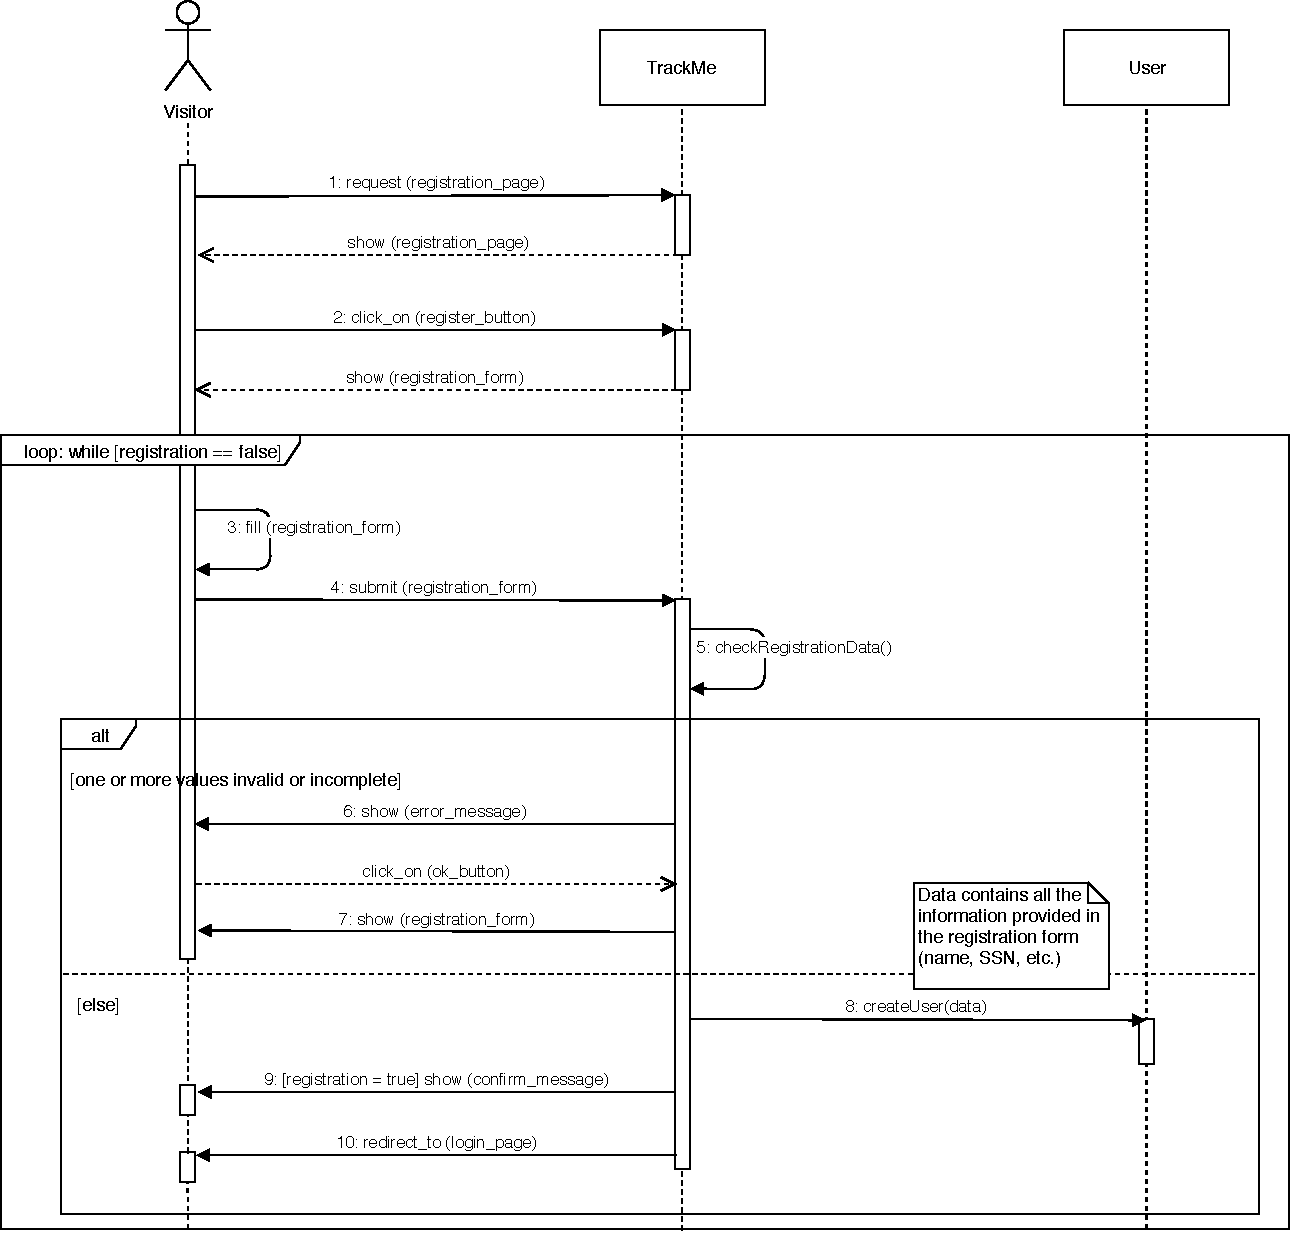
\includegraphics[width=1.25\linewidth]{Images/registration_sequence}
				\label{fig:registration_sequence}
			\end{figure}
		\subsubsection{Login}
			\begin{figure}[H]
				\centering
				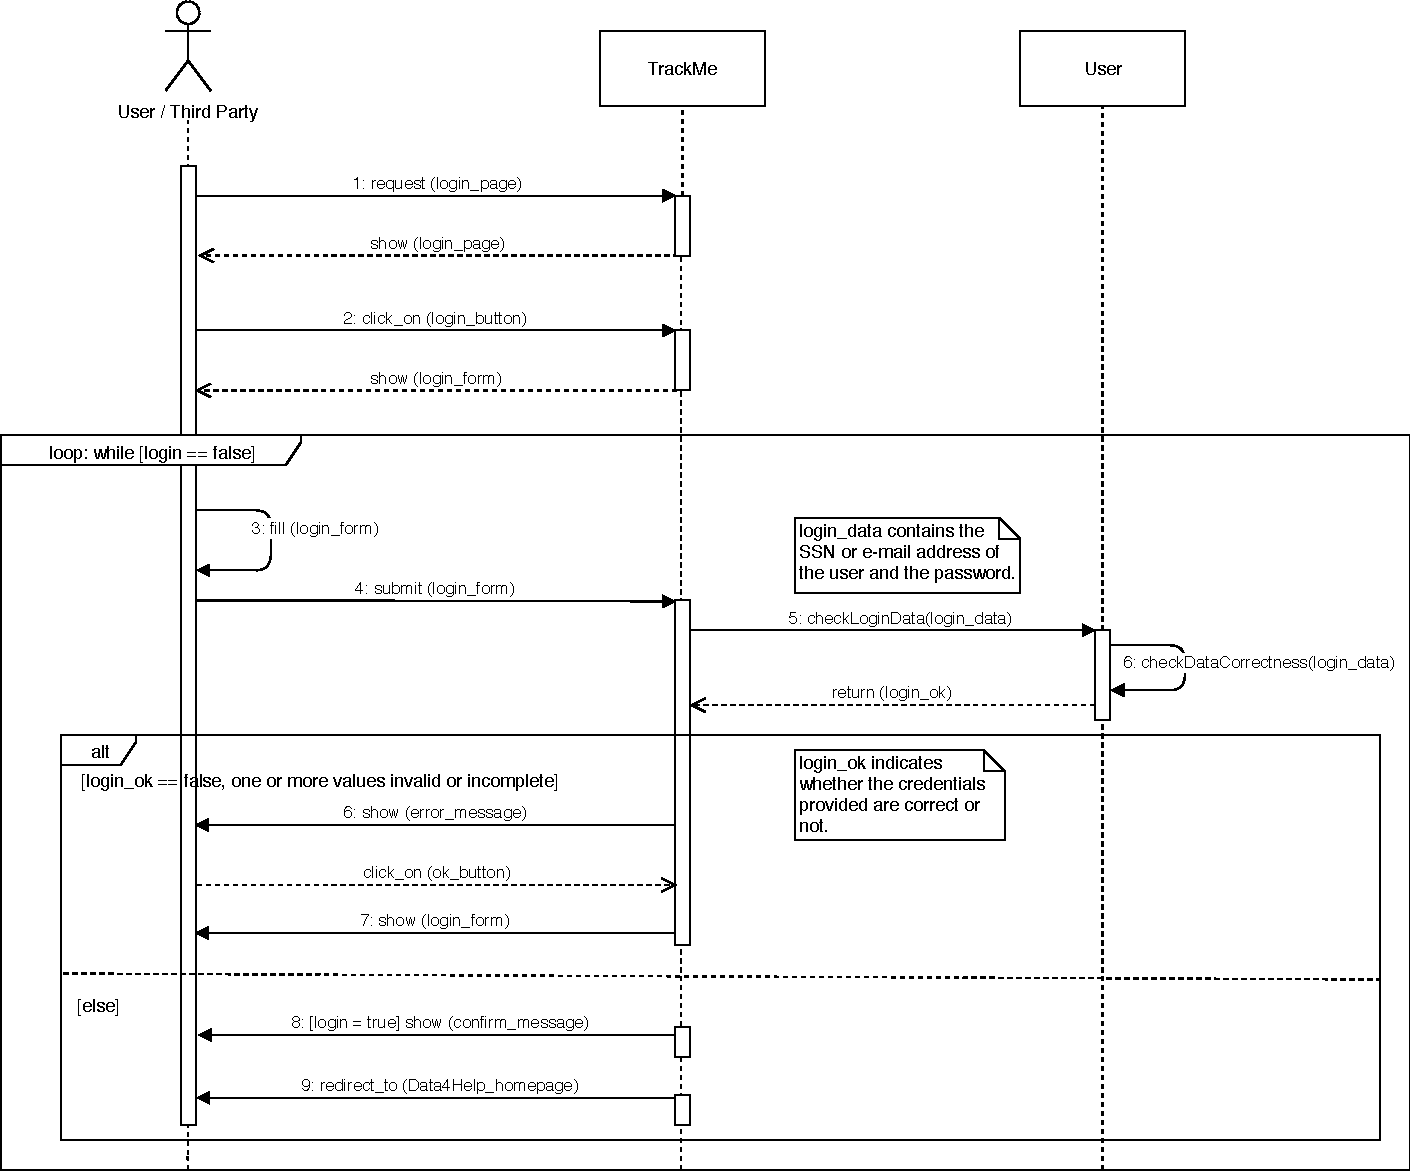
\includegraphics[width=1.2\linewidth]{Images/login_sequence}
				\label{fig:login_sequence}
			\end{figure}
		\subsubsection{User Data Access Request and Subscription}
			\begin{figure}[H]
				\centering
				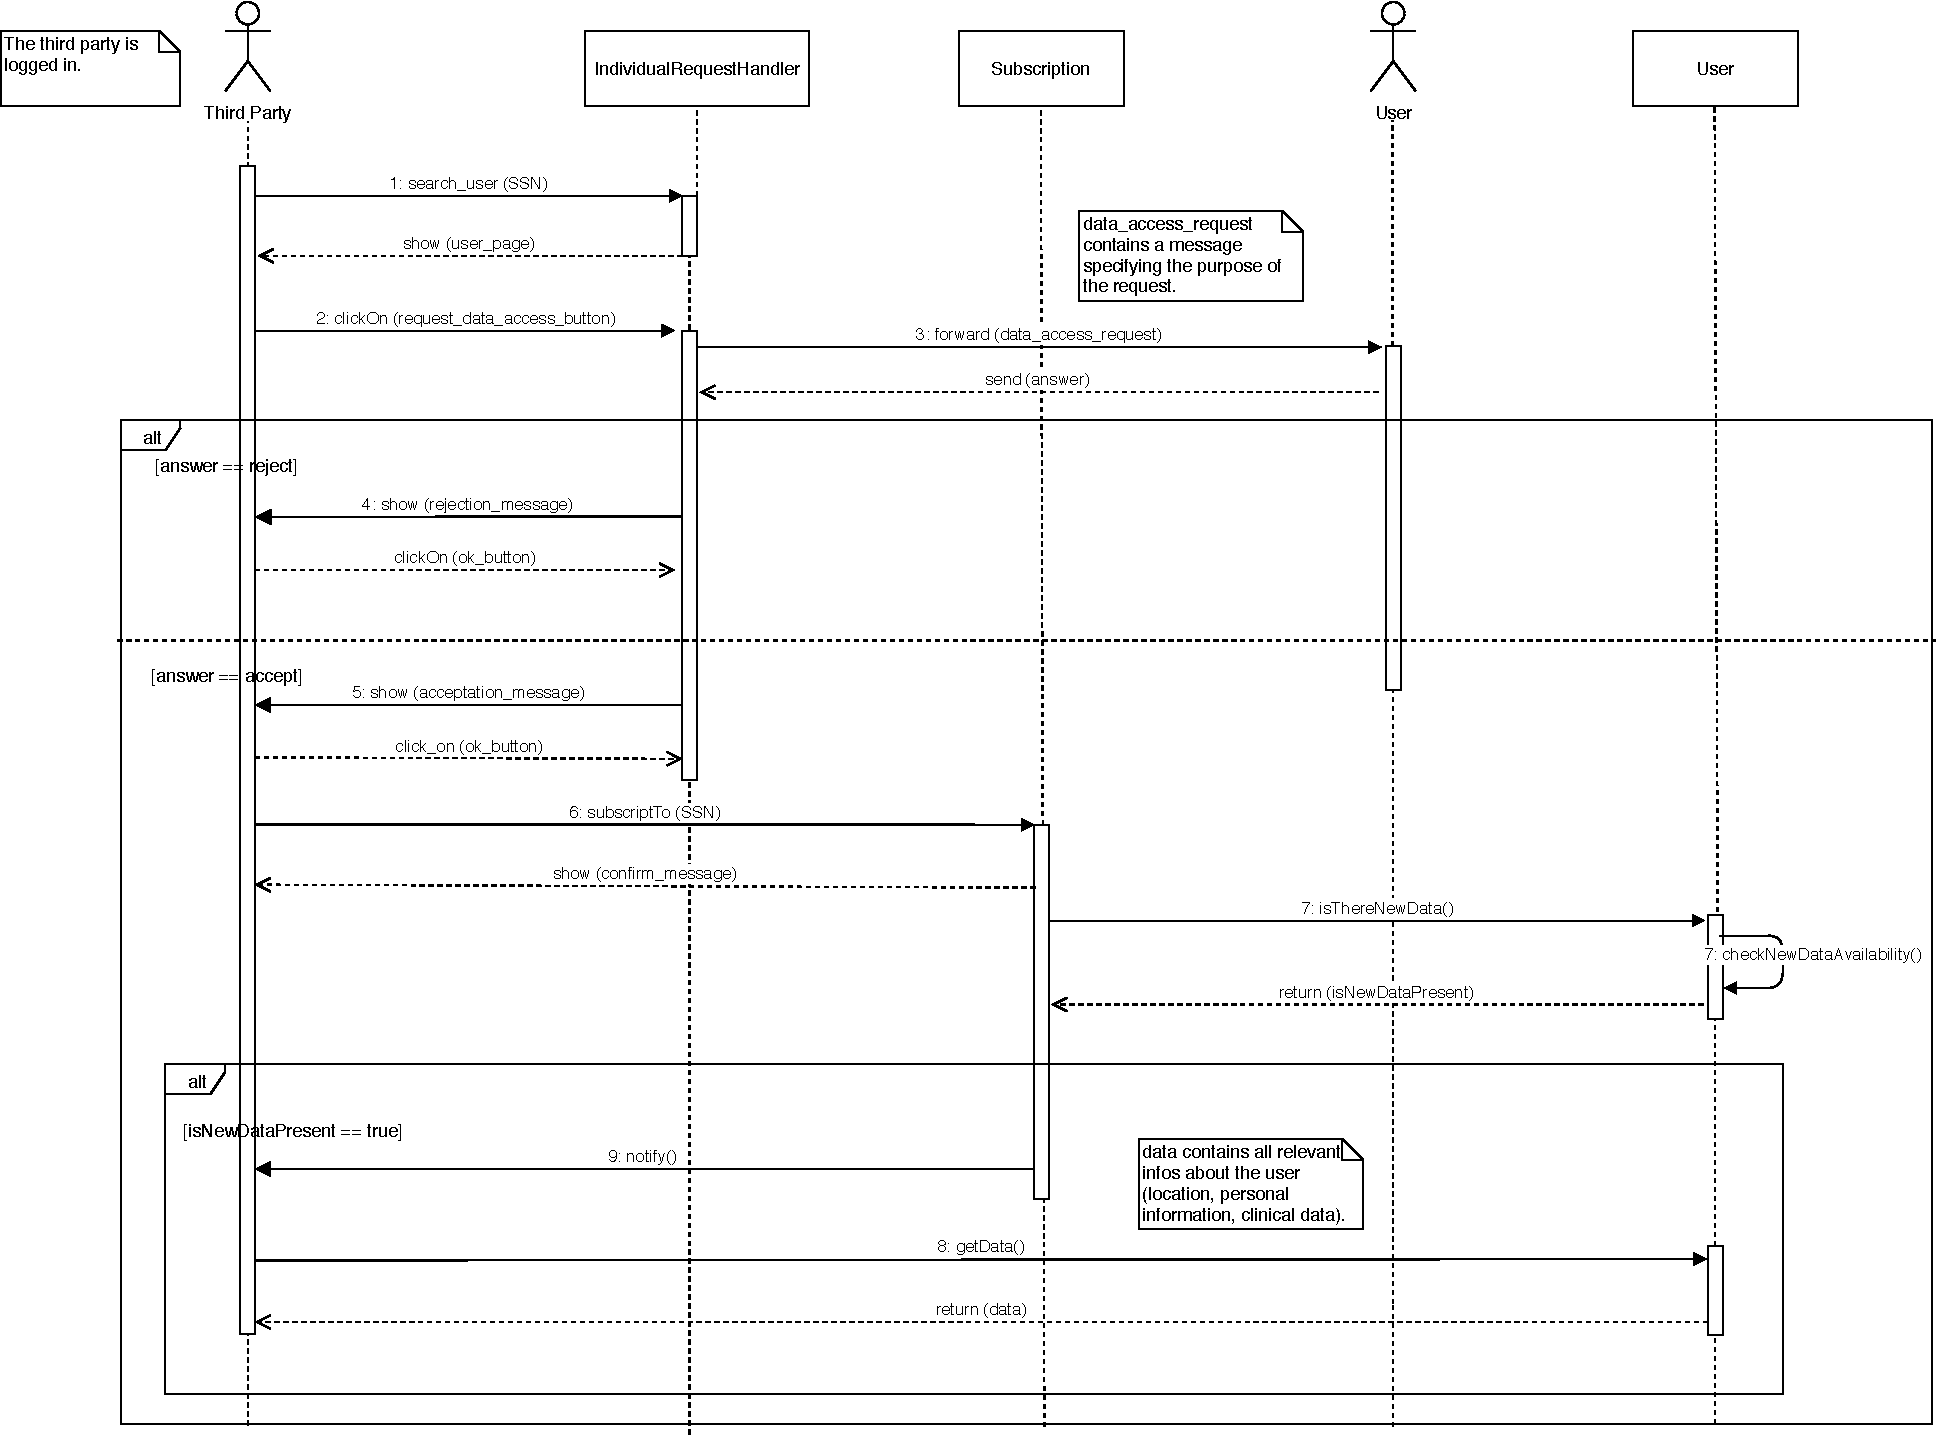
\includegraphics[width=1.2\linewidth]{Images/request_subscription_sequence}
				\label{fig:request_subscription_sequence}
			\end{figure}
		\subsubsection{On-Demand Assistance Request}
			\begin{figure}[H]
				\centering
				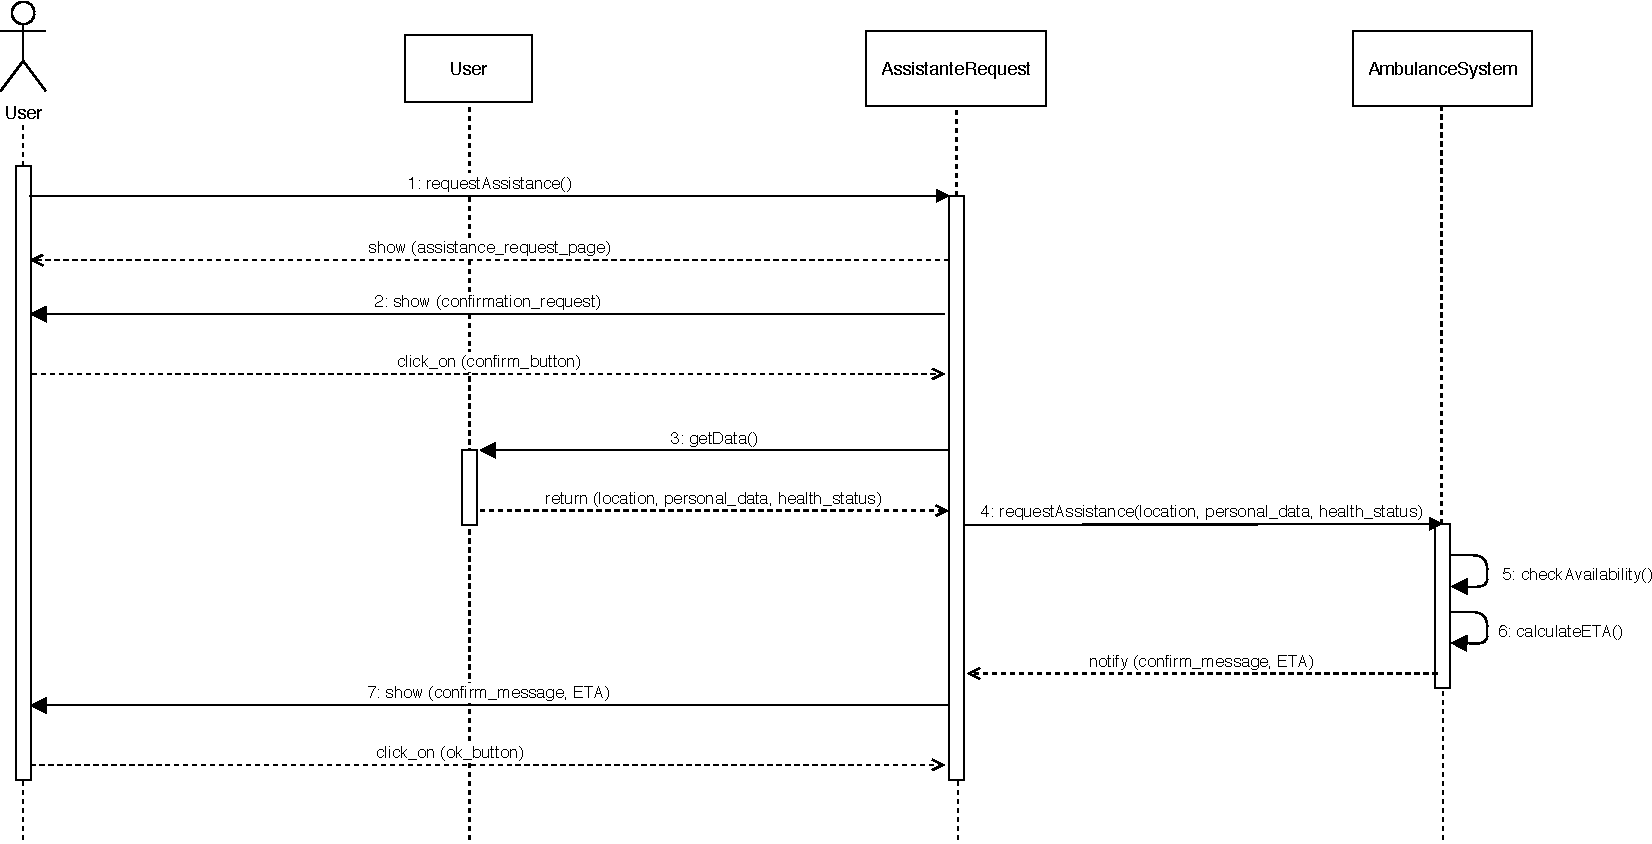
\includegraphics[width=1.1\linewidth]{Images/ass_request_sequence}
				\label{fig:ass_request_sequence}
			\end{figure}
		\subsubsection{Automated Assistance Request}
			\begin{figure}[H]
				\centering
				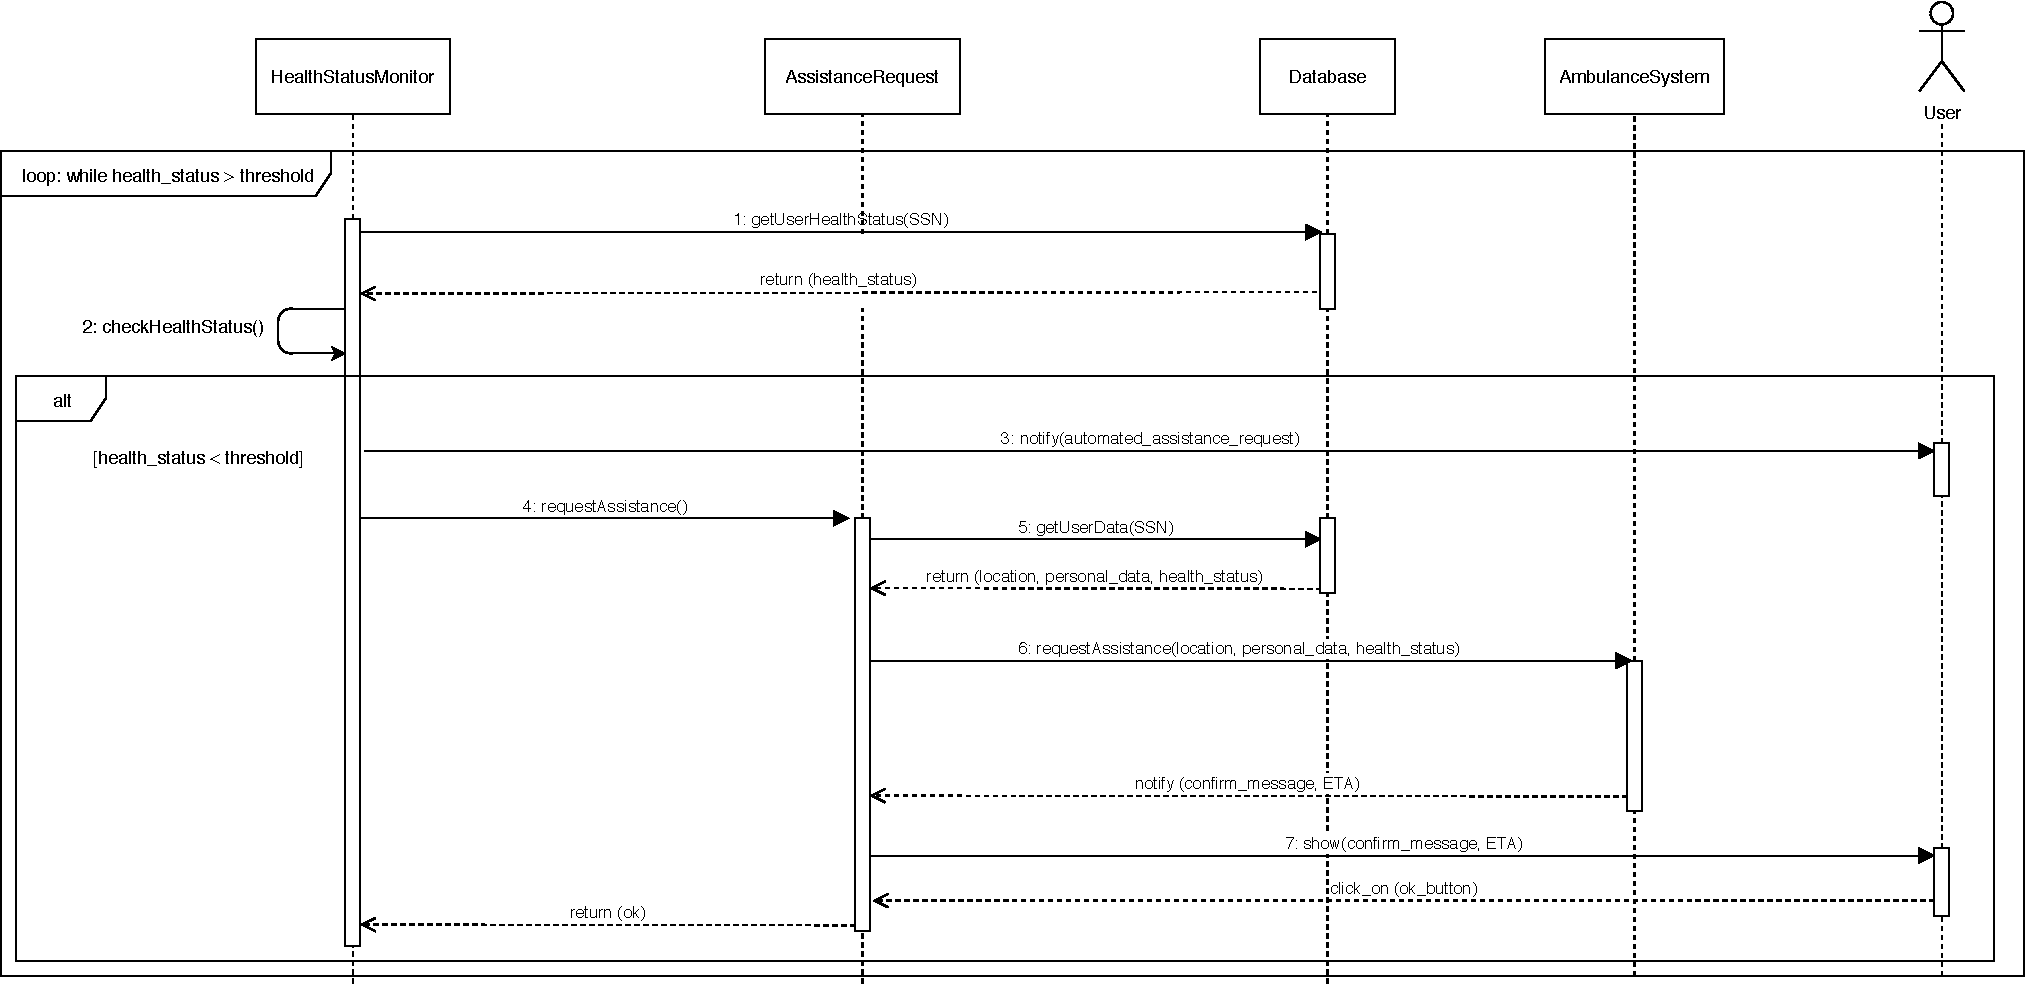
\includegraphics[width=1.1\linewidth]{Images/automated_request_sequence}
				\label{fig:automated_request_sequence}
			\end{figure}
		\subsubsection{Sampling Search}
			\begin{figure}[H]
				\centering
				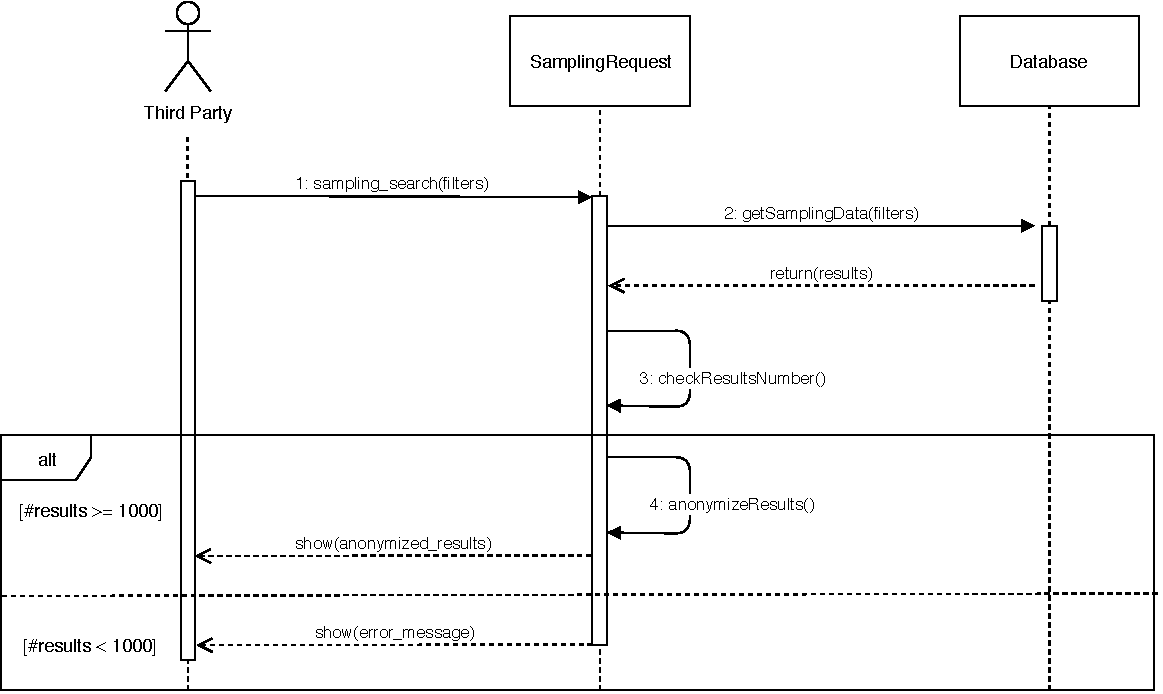
\includegraphics[width=1.2\linewidth]{Images/sampling_request_sequence}
				\label{fig:sampling_request_sequence}
			\end{figure}

	\subsection{Performance Requirements}
	The system must be able to handle a huge quantity of requests simultaneously throughout the day, responding to users' necessities in the shortest time possible. In order to improve the performance of the system, since data are received in a discrete way (e.g. monitored every 5 seconds), TrackMe should rely on lightweight TCP connections.\\
	For what concerns the AutomatedSOS service, it is required that each ambulance request is generated and sent to the Ambulance Dispatching System within 5 seconds from the moment in which the vital parameters of a user subscribed to this service get below the fixed threshold.

	\newpage
	\subsection{Design Constraints}
	\subsubsection{Hardware Limitations}
		\begin{itemize}
			\item \texttt{Mobile App}: 
				\begin{itemize}
					\item Smartphones: iOS/Android, Internet Connection, GPS.
					\item Smartwatches: watchOS/WearOS with hearbeat/pressure sensors linked to mobile devices or equipped with GPS and internet connectivity.
				\end{itemize}
			\item \texttt{Web App}: modern web browser (e.g. Google Chrome / Safari), able to support the already mentioned communication protocols and APIs.
		\end{itemize}
	
	%\subsubsection{Other Constraints}

	\subsection{Software System Attributes}
		\subsubsection{Reliability}
		The system must guarantee a 24/7 service. This requirment should not have any sort of deviation (especially concerning AutomatedSOS).
		\subsubsection{Availability}
		The system must fullfil all the requests whenever needed (e.g. get/update personal information, request for medical assistance). Only a small percentage of the total requests is admissible (less than 0.01\% of the total amount of requests). The system relies on a RAPS architecture (see more in depth in the Design Document, section 2.6.2), to better guarantee availability.
		\subsubsection{Security}
		Despite the fact that personal information is stored, the system guarantees not to spread them outside, and third parties are obliged to be confirmed with a privacy policy.
		\subsubsection{Maintainability}
		Enforced by the usage of specific design patterns (e.g. third party subscription is notified through an Observer Pattern whenever new data is generated by the users) and the provided documentation.
		\subsubsection{Scalability}
		The architecture must be simply scalable as the number of users grows during the time.
		 Enlarging the structure of the system must be an easy task, having the possibility to invest only on those services that need to handle the higher amount of requests or the ones where the number of users is relevant.


	\newpage
	\section{Formal Analysis Using Alloy}
		\subsection{Purpose of the Model}
			Through this model we want to formalize some principal aspects of the TrackMe system:
			\begin{itemize}
				\item All the users that receive an automated assistance are necessarily subscribed to the AutomatedSOS service. 
				Furthermore, users cannot receive multiple assistances at the same time and an automatic assistance is generated 
				whenever his/her health status gets below the critical threshold (here represented by 0). All the users with an age grater or equal to 60 (here represented by 6) are automatically registered to AutomatedSOS, but this doesn't preclude younger users to subscribe to the service too. If an automated assistance request is generated, then it must be sent to the Ambulance System within 5 seconds.
				\item All the third parties in order to have access to some users' data, have to send a request to the specific user, that can be either accepted or rejected. Only if the user accepts the request, then the third party can access all his/her data. If the access is granted, then the third party has the possibility to subscribe to user's new data (but it is not necessary).
				\item Third Parties have the possibility to do sample searches according to some filters. TrackMe validates only those searches that result in more than 1000 users (here represented by 1). 
			\end{itemize}
		\subsection{Alloy Model}
			\begin{figure}[H]
				\centering
				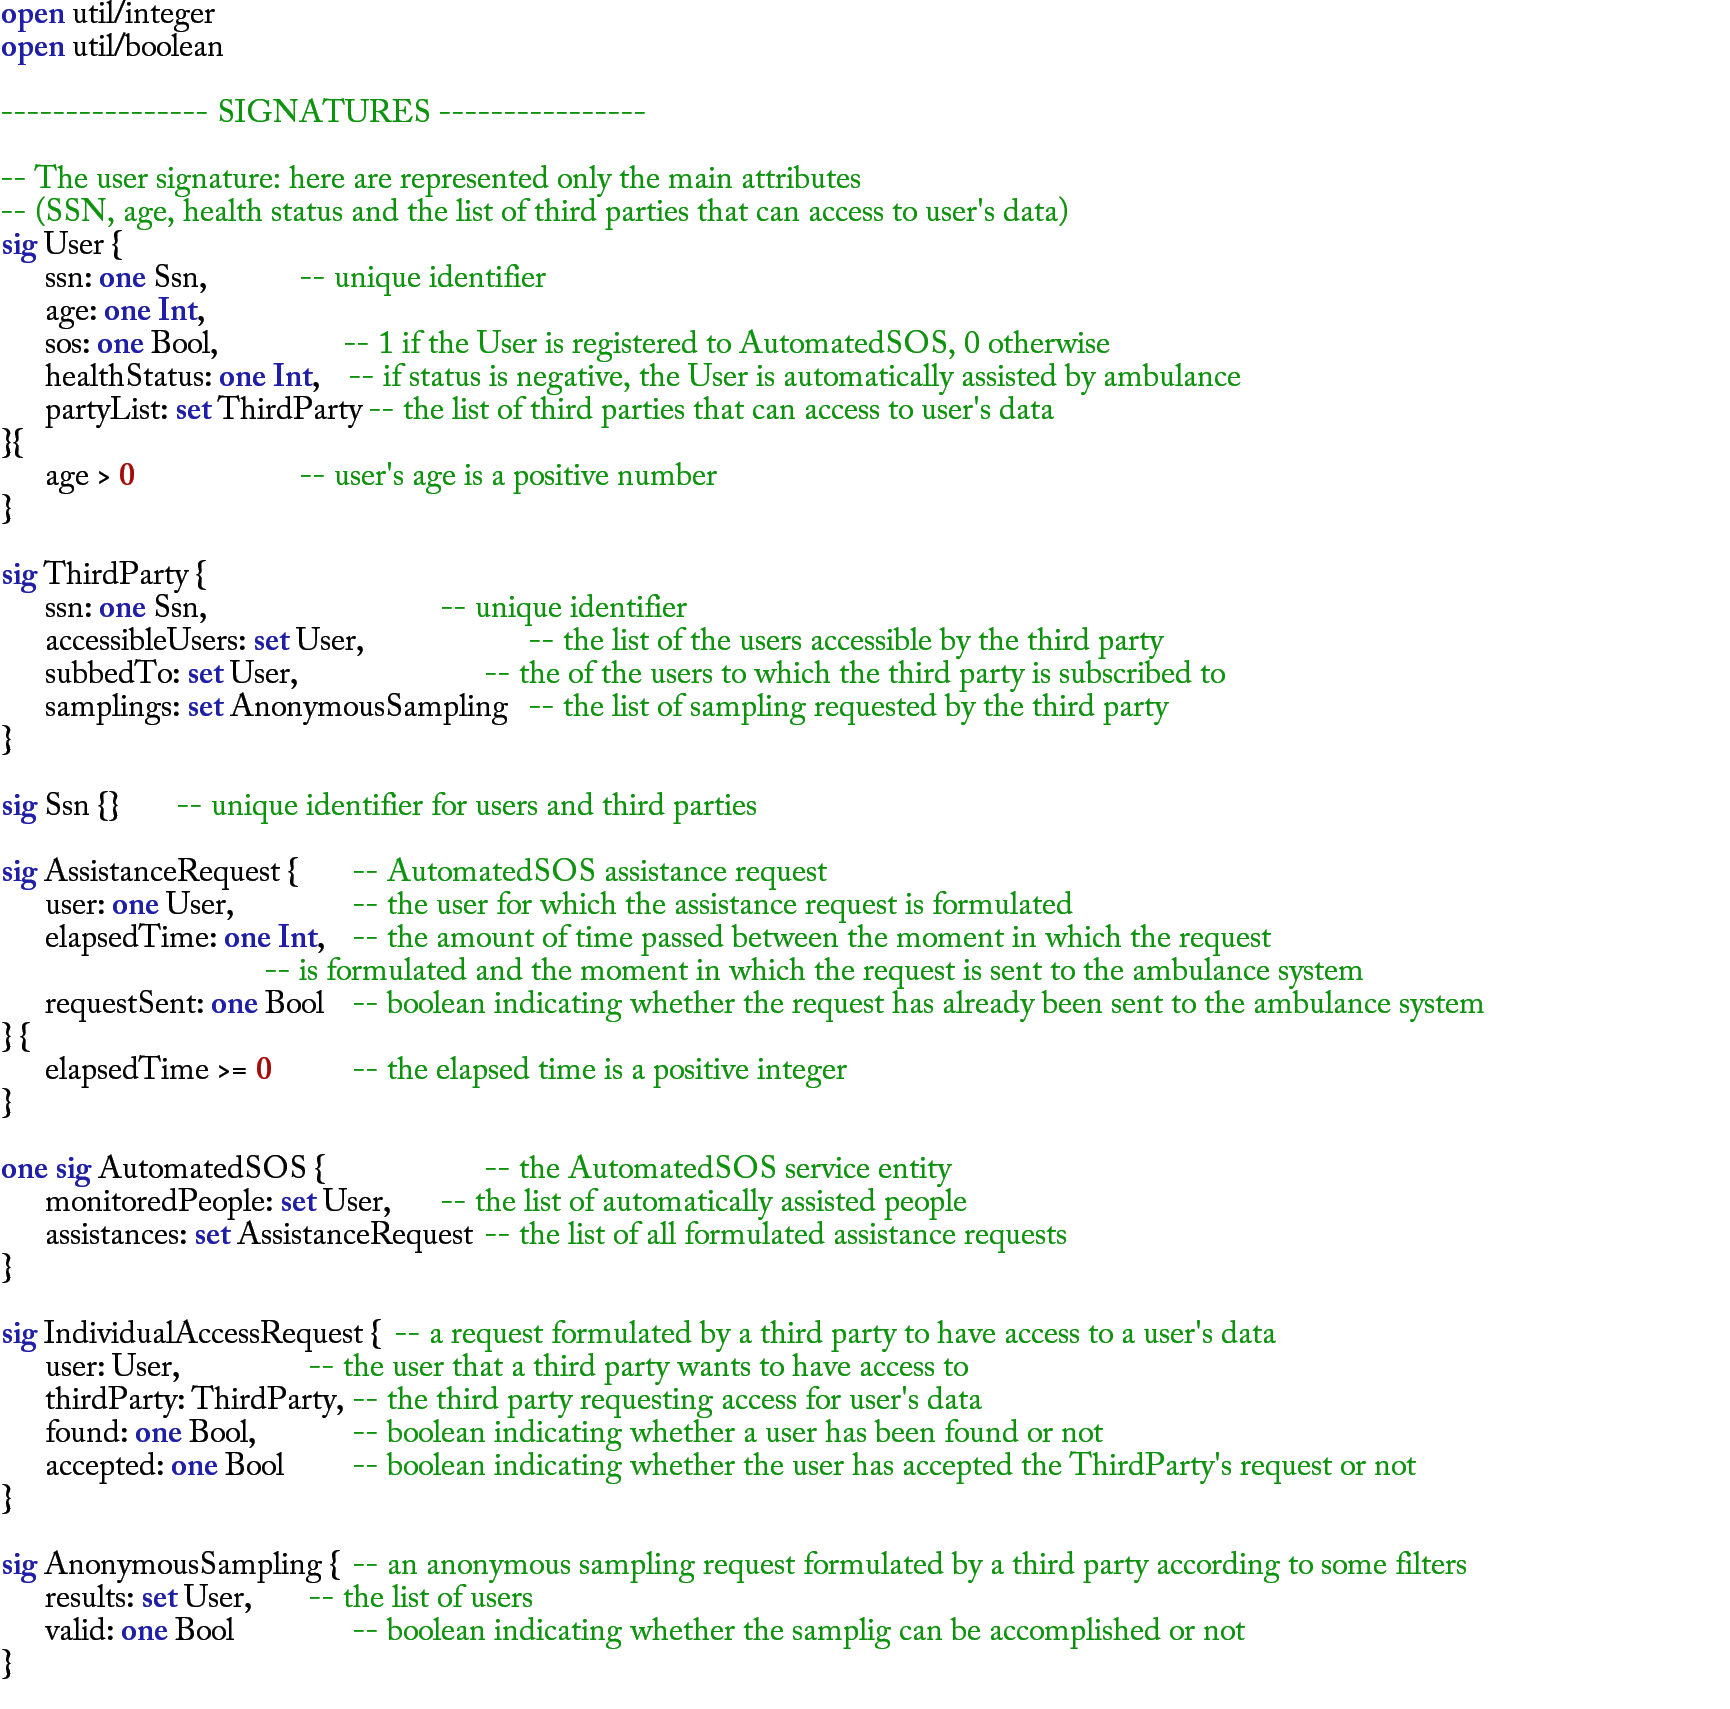
\includegraphics[width=1.4\linewidth]{Images/signatures}
				\label{fig:signatures}
			\end{figure}
			\begin{figure}[H]
				\centering
				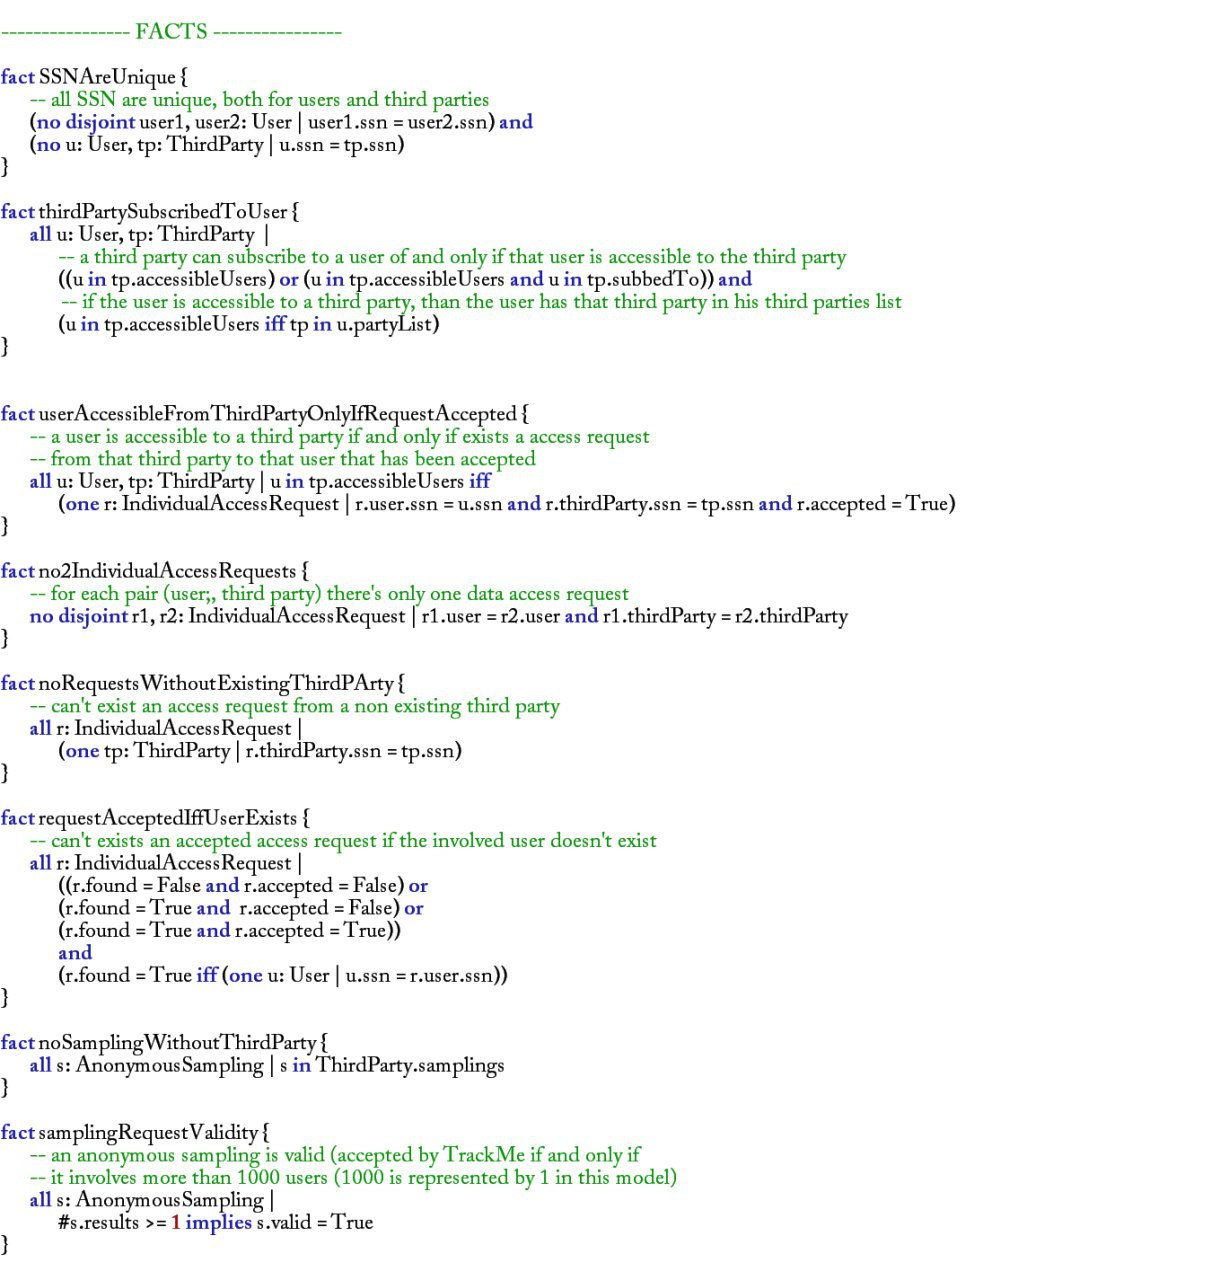
\includegraphics[width=1.3\linewidth]{Images/facts1}
				\label{fig:facts1}
			\end{figure}
				\begin{figure}[H]
				\centering
				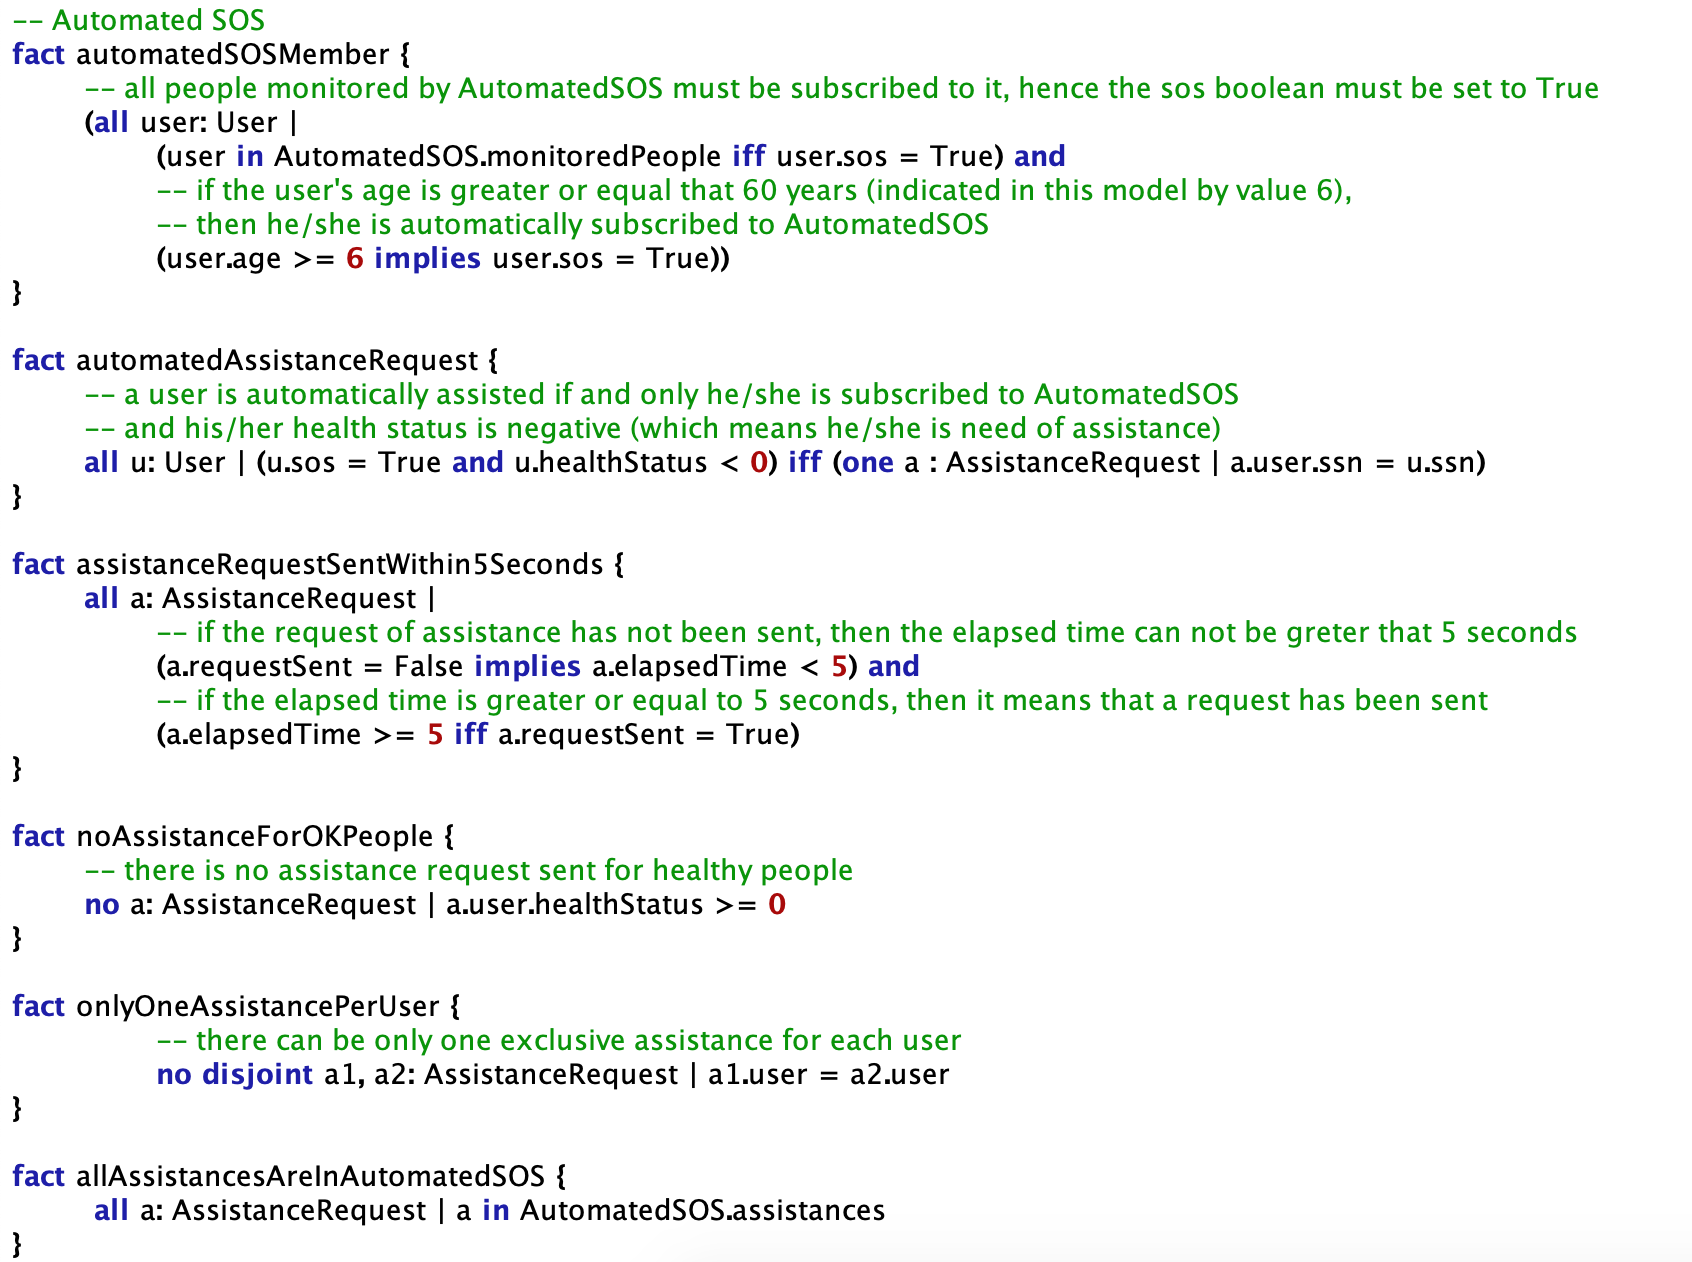
\includegraphics[width=1.3\linewidth]{Images/facts2}
				\label{fig:facts2}
			\end{figure}
			\begin{figure}[H]
				\centering
				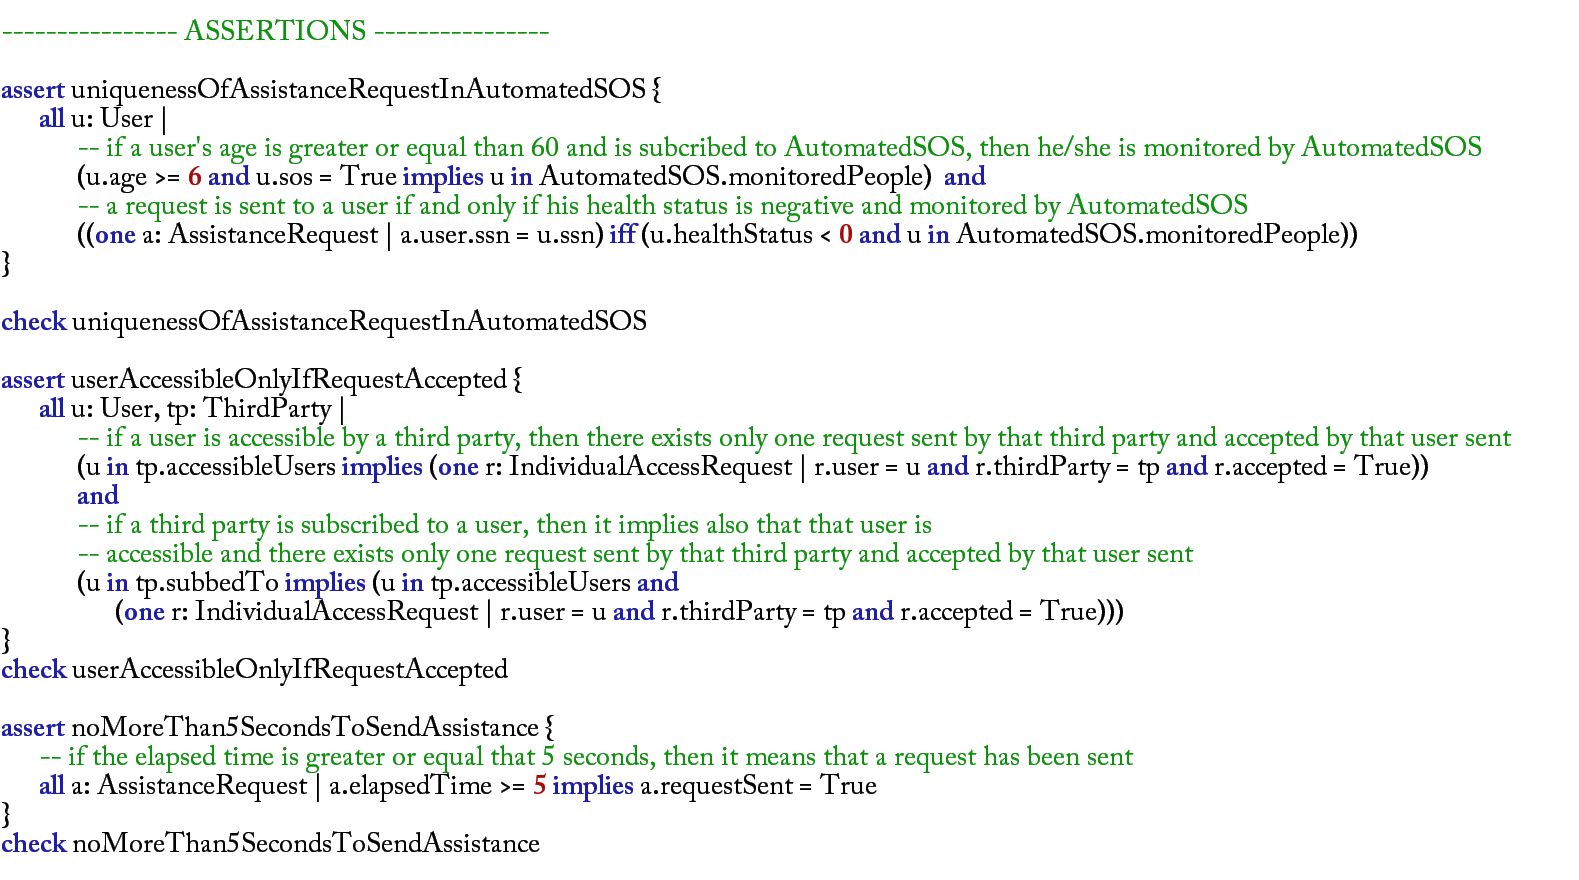
\includegraphics[width=1.3\linewidth]{Images/assertions}
				\label{fig:assertions}
			\end{figure}
			\begin{figure}[H]
				\centering
				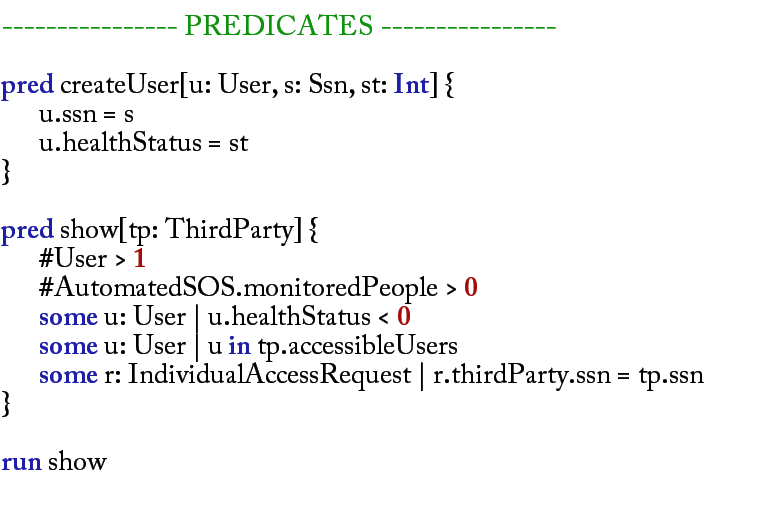
\includegraphics[width=0.7\linewidth]{Images/predicates}
				\label{fig:predicates}
			\end{figure}
			\begin{figure}[H]
				\centering
				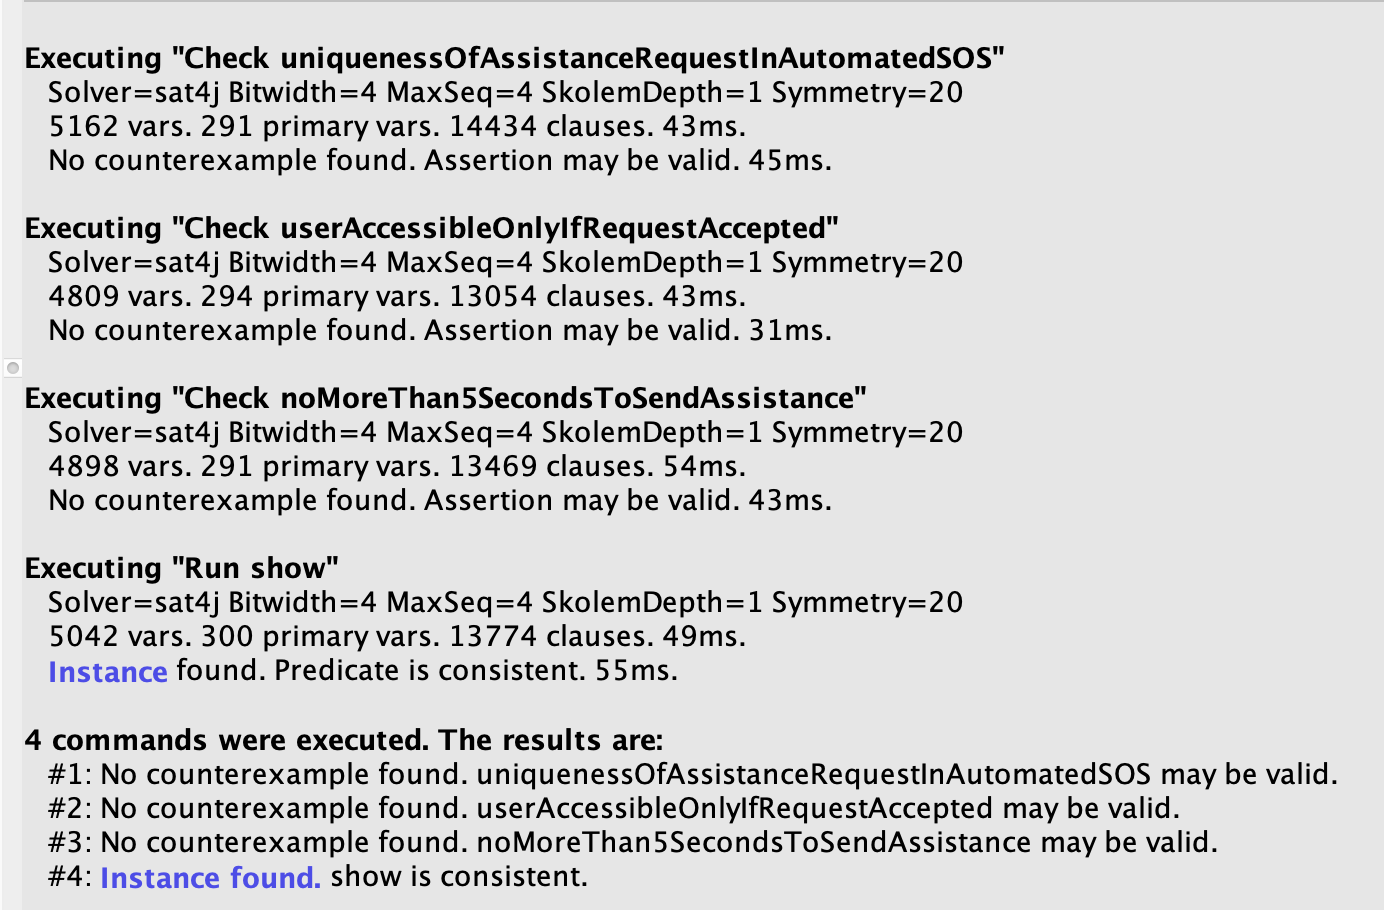
\includegraphics[width=1.2\linewidth]{Images/alloy-consistency}
				\label{fig:alloy-consistency}
			\end{figure}
	\newpage
	\subsection{Generated World}
		\subsubsection{First Instance}
			As can be seen from this instance there are two different users, but only User1 is monitored by AutomatedSOS, since his age is equal to 7 (greater than 6). In addition his health status is negative and there exist an AssistanceRequest that has already been sent (the elapsed time equals to 5). 
			Moreover, there's a Third Party that has access to both of the users' data, but it is subscribed only to User0. This situation is possible thanks to the two accepted IndividualAccessRequest sent by the Third Party to both the users.\\
			\begin{figure}[H]
				\centering
				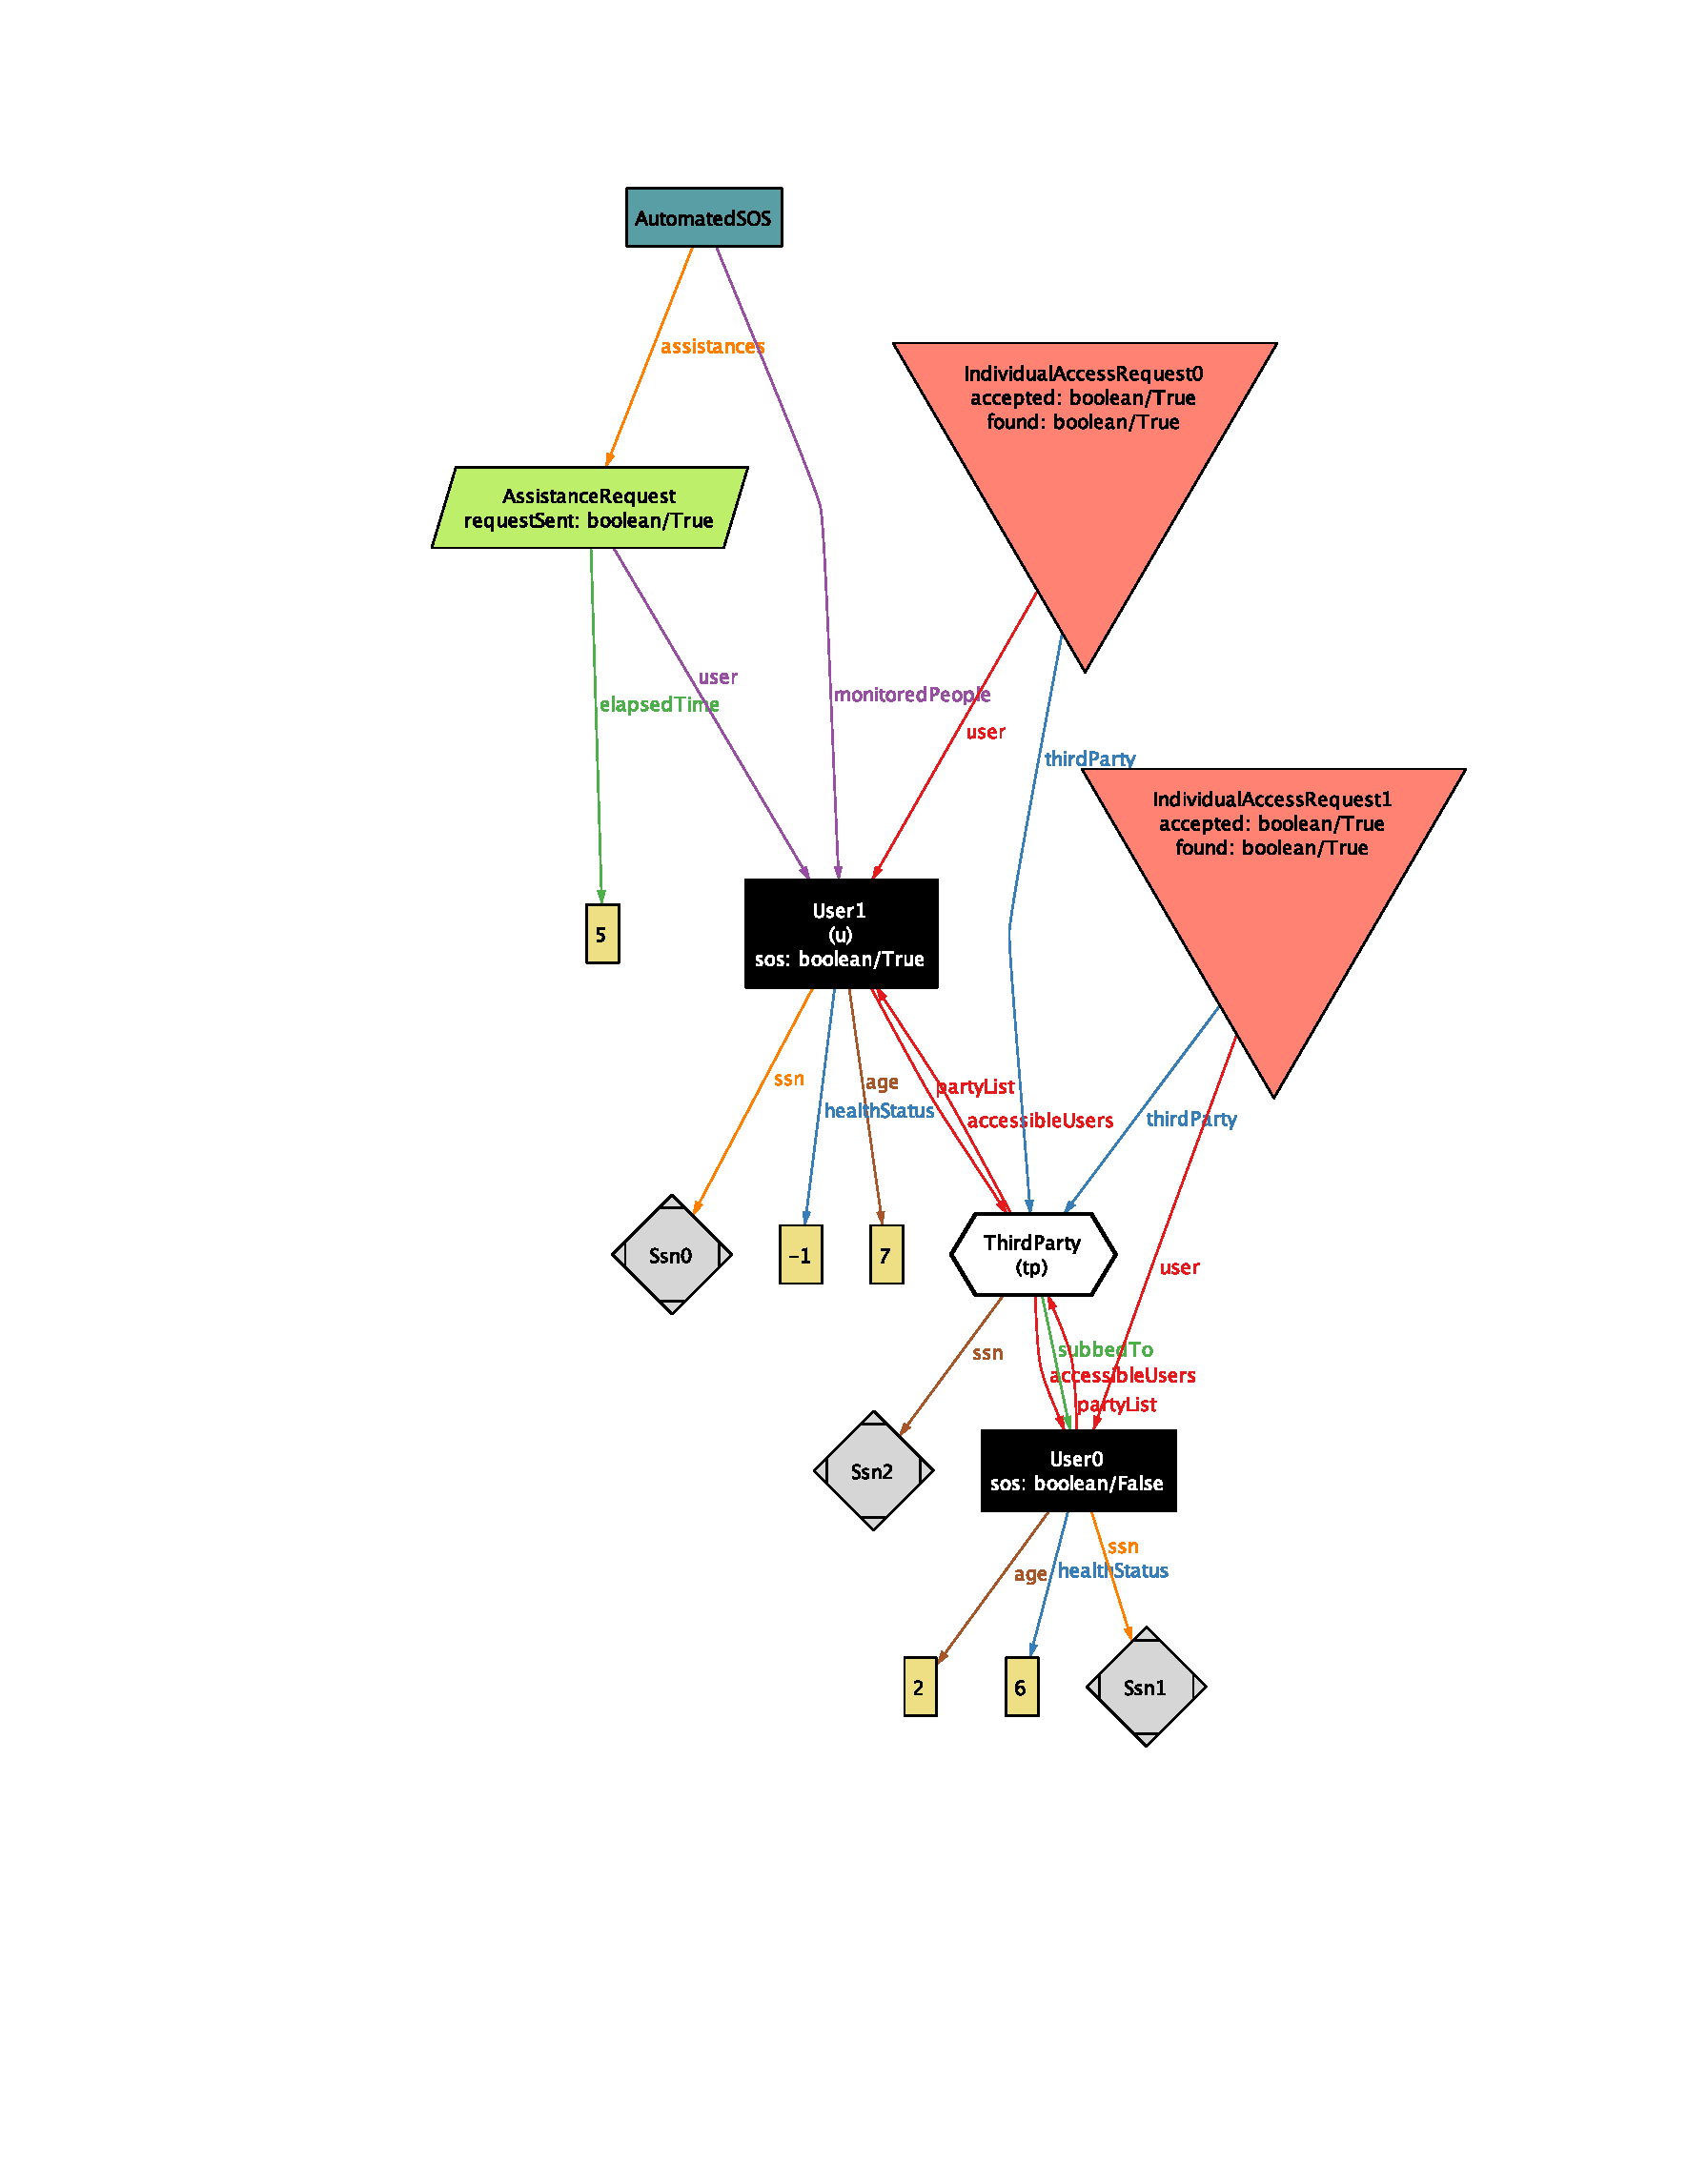
\includegraphics[height=1.0\linewidth]{Images/first-world}
				\label{fig:first-world}
			\end{figure}
		\subsubsection{Second Instance}
			The illustrated situation is similar to the previous one, even though both users are monitored by AutomatedSOS (one has age greater than 6, the other one doesn't). 
			In addition three different sampling searches have been generated. AnonymousSampling2 is valid, since it contains in its results list both User0 and User1 (\#results is greater than 1). The other two samplings are not validated by TrackMe because they don't respect the privacy policies the system is based on (\#results equals 0).\\
			\begin{figure}[H]
				\centering
				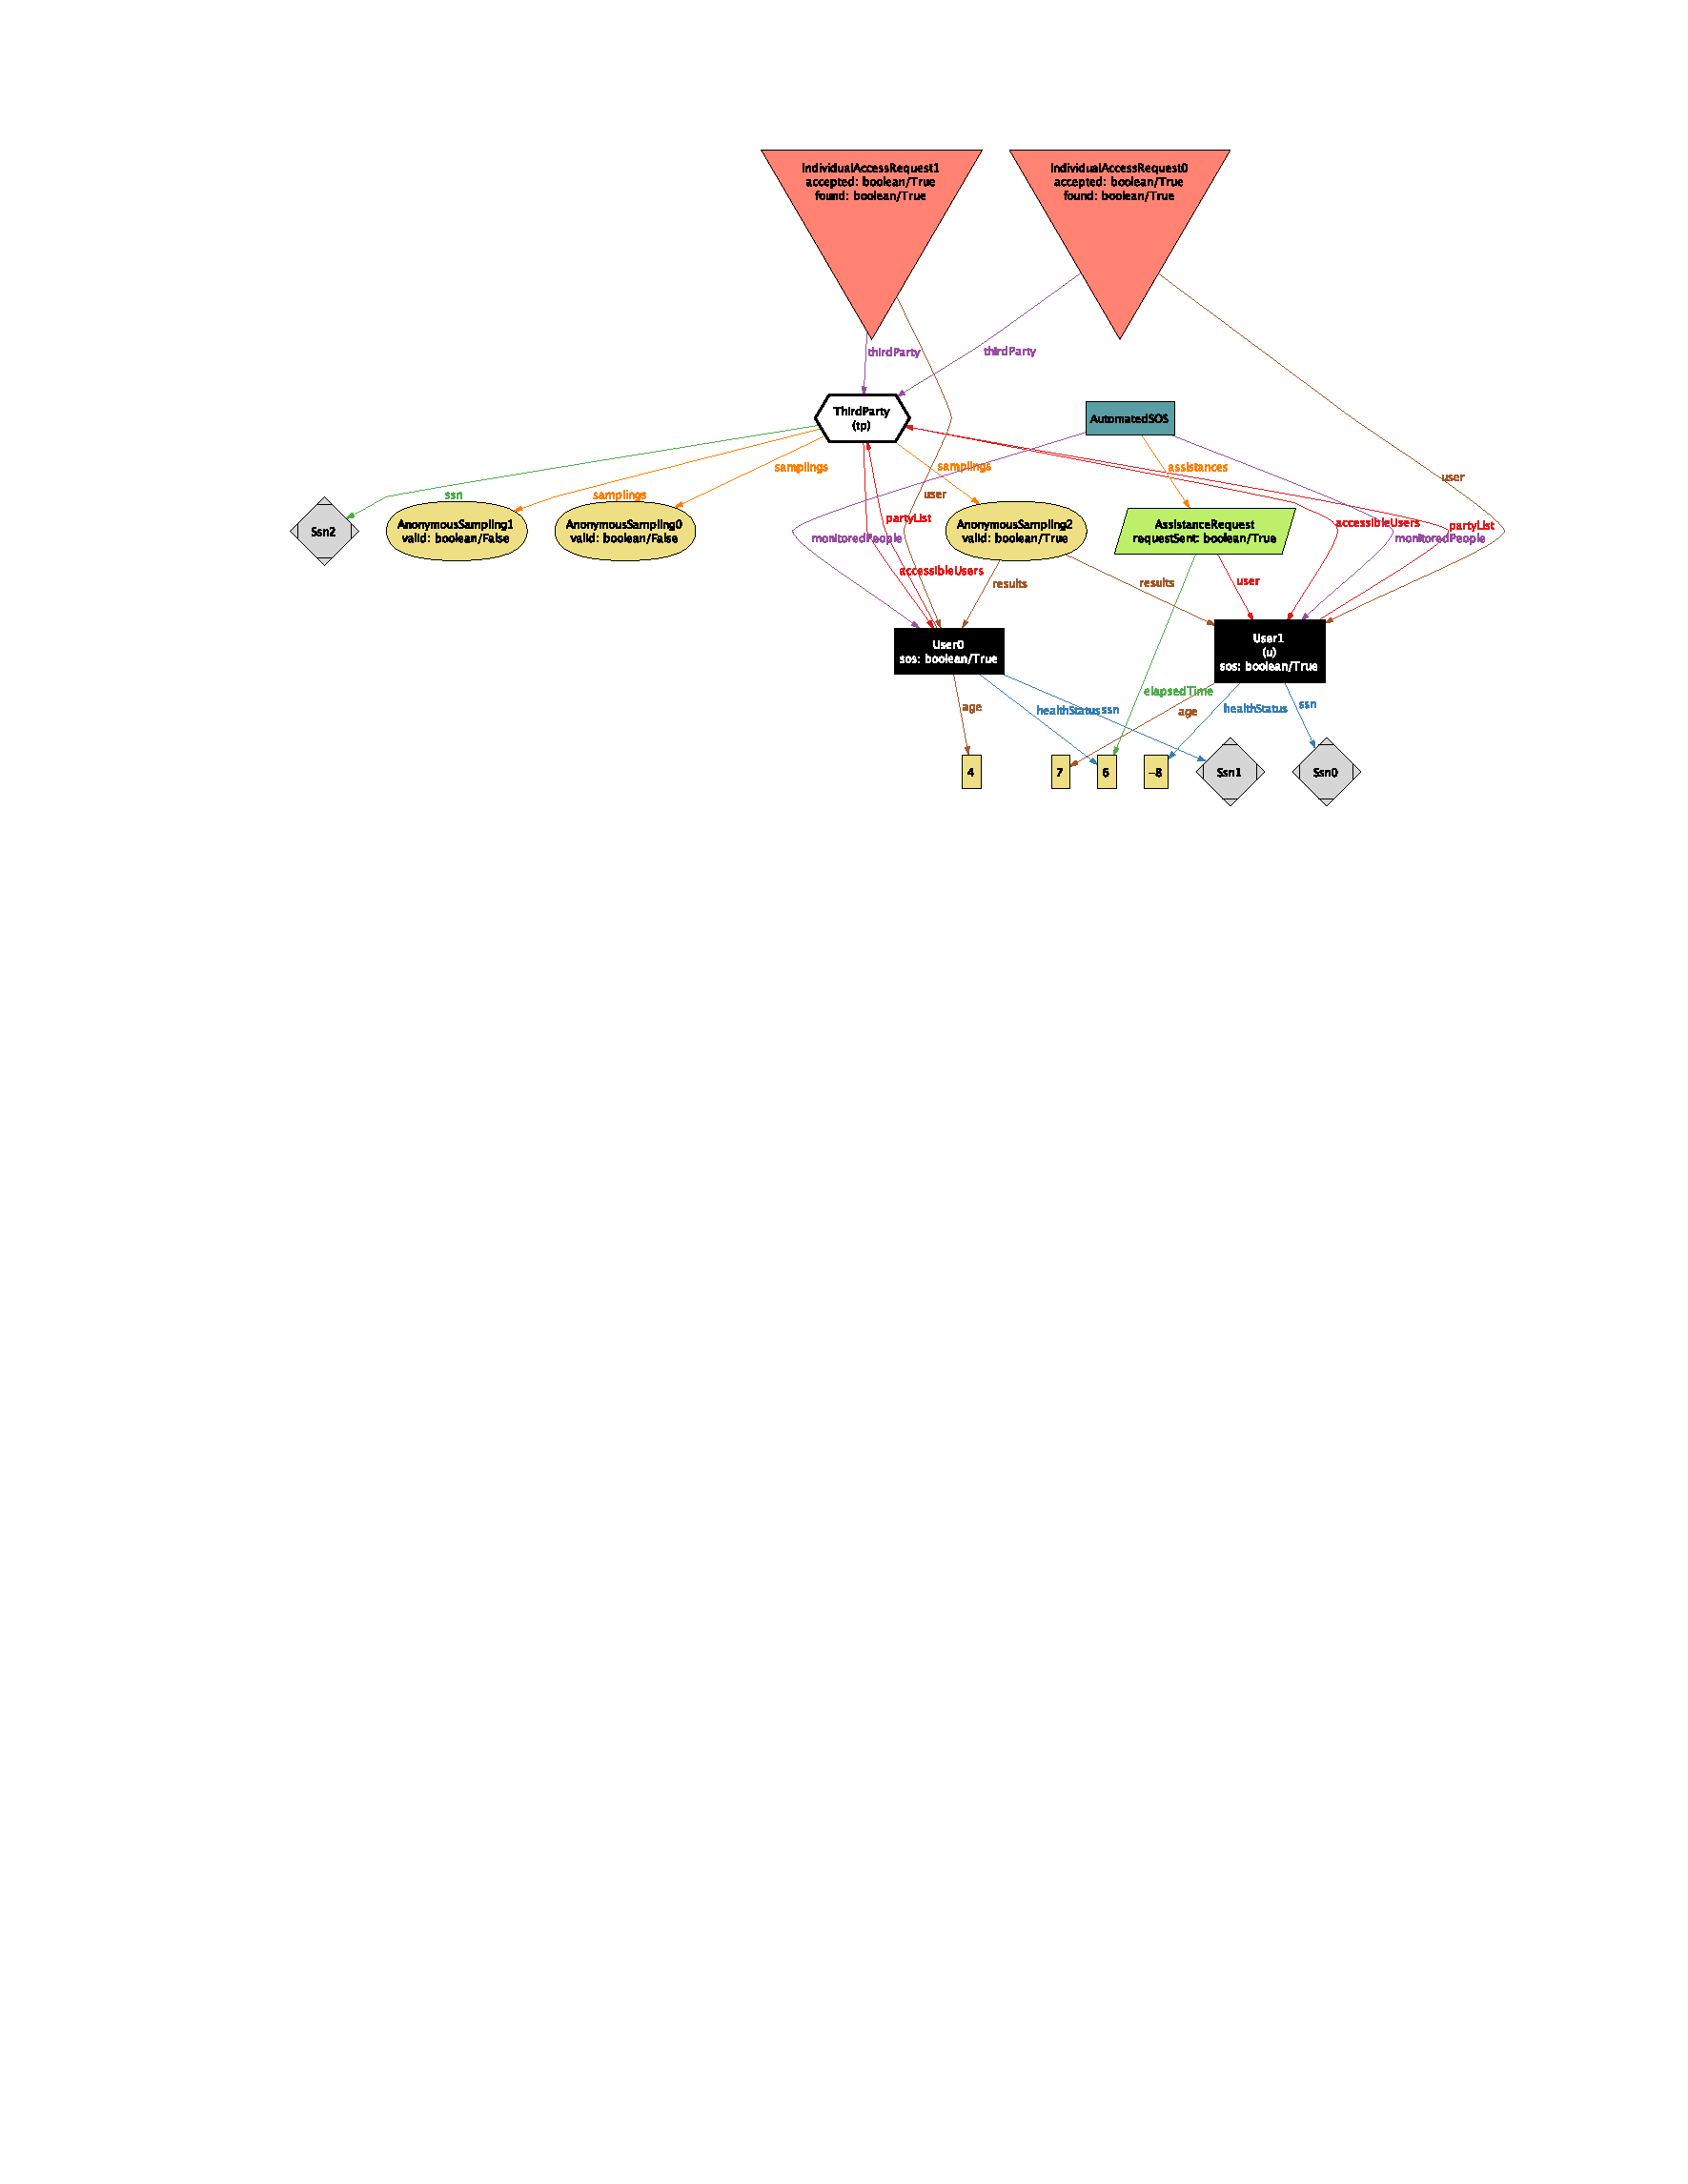
\includegraphics[width=1.25\linewidth]{Images/second-world}
				\label{fig:second-world}
			\end{figure}

	\newpage
	%\section{Appendix}
	%\subsection{Tools used}

	\section{Effort Spent}
	\begin{itemize}
		\item Luca Conterio
		\begin{center}
			\begin{tabular}{| c | c | c |}
				\hline
				Day & Subject & Hours \\ \hline
				15/10/2018 & Purpose, Scope and goals & 1 \\
				18/10/2018 & Overall Description & 1.5 \\
				19/10/2018  & User Interface sketch and Domain Assumptioms & 2 \\
				22/10/2018  & UML and Non-Functional Requirements & 3.5 \\
				25/10/2018 & Functional Requirements & 3 \\
				26/10/2018 & Statechart Diagrams & 2 \\
				28/10/2018 & User Interface and Scenarios & 1.5 \\
				29/10/2018 & Interfaces and Scenarios & 1.5 \\
				03/11/2018 & Sequence Diagrams & 2 \\
				07/11/2018 & Sequence Diagrams & 2 \\
				08/11/2018 & Alloy Model & 3 \\
				09/11/2018 & Alloy Model & 4 \\
				11/11/2018 & Alloy Comment and General Revision & 4 \\
				\hline
				Total & & 31 \\
				\hline
			\end{tabular}
		\end{center}

		\item Ibrahim El Shemy
		\begin{center}
			\begin{tabular}{| c | c | c |}
				\hline
				Day & Subject & Hours \\ \hline
				15/10/2018 & Purpose, Scope and goals & 1 \\
				18/10/2018 & Overall Description and Product Functions & 2 \\
				19/10/2018  & Domain Assumptions & 2 \\
				22/10/2018  & Assumptions and Non-Functional Requirements & 3.5 \\
				25/10/2018 & Functional Requirements & 3 \\
				26/10/2018 & Functional Requirements & 1 \\
				27/10/2018 & Use Case Diagram & 3 \\
				28/10/2018 & Use Case Diagram and Use Cases & 1 \\
				02/11/2018 & Scenarios Review and Use Cases & 1.5 \\
				07/11/2018 & Alloy Model & 1.5 \\
				08/11/2018 & Alloy Model & 3 \\
				09/11/2018 & Alloy Model & 3 \\
				11/11/2018 & Alloy Comment and General Revision & 4 \\
				\hline
				Total & & 29.5 \\
				\hline
			\end{tabular}
		\end{center}
	\end{itemize}
	\section{References and Used Tools}
		\subsection{Reference Documents}
			\begin{itemize}
				\item Specification Document "Mandatory Project Assignment A.Y. 2018/2019"
				\item 830-1993 - IEEE Recommended Practice for Software Requirements
				\item "Appunti di Sistemi Informativi per il Settore dell'Informazione" A.Y. 2017/2018
				\item Alloy Language Reference "http://alloytools.org/download/alloy-language-reference.pdf"
			\end{itemize}
		
		\subsection{Tools}
			\begin{itemize}
				\item \textbf{Draw.io}: \texttt{https://www.draw.io/}
				\item \textbf{TeXstudio}: \texttt{http://www.textstudio.org/}
				\item \textbf{Github}: \texttt{https://github.com/}
			\end{itemize}
\end{document}
